%; whizzy paragraph
%; whizzy-paragraph "^\\\\dancersection"
% -initex iniptex -latex platex -format platex -bibtex jbibtex -fmt fmt
% $B0J>e(B whizzytex $B$r;HMQ$9$k>l9g$N@_Dj!#(B

%     Tokyo Debian Meeting resources
%     Kansai Debian Meeting resources
%     Copyright (C) 2012 Junichi Uekawa
%     Copyright (C) 2012 Nobuhiro Iwamatsu
%     Copyright (C) 2012 Koichi Akabe

%     This program is free software; you can redistribute it and/or modify
%     it under the terms of the GNU General Public License as published by
%     the Free Software Foundation; either version 2 of the License, or
%     (at your option) any later version.

%     This program is distributed in the hope that it will be useful,
%     but WITHOUT ANY WARRANTY; without even the implied warranty of
%     MERCHANTABILITY or FITNESS FOR A PARTICULAR PURPOSE.  See the
%     GNU General Public License for more details.

%     You should have received a copy of the GNU General Public License
%     along with this program; if not, write to the Free Software
%     Foundation, Inc., 51 Franklin St, Fifth Floor, Boston, MA  02110-1301 USA

%  preview (shell-command (concat "evince " (replace-regexp-in-string "tex$" "pdf"(buffer-file-name)) "&"))
% $B2hA|%U%!%$%k$r=hM}$9$k$?$a$K$O(Bebb$B$rMxMQ$7$F(Bboundingbox$B$r:n@.!#(B
%(shell-command "cd image2012-natsu; ebb *.png")

% progress memo:
% 2017/12-2018/06$BEl5~$,%^!<%8BP>](B
% $B%$%Y%s%HEy$G$J$$>l9g$OM}M3$r=q$/$3$H!#(B
% $BI,MW$JJQ99E@$O(B FIXME $B$G5-O?$7$F$$$^$9!#(B

%%$B$3$3$+$i%X%C%@3+;O!#(B

\documentclass[mingoth,a4paper]{jsarticle}
\usepackage{monthlyreport}
\usepackage{supertabular}
\usepackage{subfigure}
\renewcommand*\thesubfigure{}

\usepackage{comment}

% section $B$NBe$o$j$N4D6-(B -- $B2~D{$9$k!#(B
\renewcommand{\dancersection}[2]{%
\newpage
$B$"$s$I$-$e$a$s$F$C$I(B $B$G$S$"$s(B 2018$BG/2F9f(B
%
% top line
\vspace{0.1mm}\\
{\color{dancerdarkblue}\rule{\hsize}{2mm}}

%
% middle text
%
\begin{minipage}[t]{0.6\hsize}
\color{dancerdarkblue}
\vspace{1cm}
\section{#1}
\hfill{}#2\\
\end{minipage}
\begin{minipage}[t]{0.4\hsize}
\vspace{-2cm}
\hfill{}
\includegraphics[height=8cm]{image200502/openlogo-nd.eps}\\
\vspace{-5cm}
\end{minipage}
%
% bottom line
{\color{dancerlightblue}\rule{0.66\hsize}{2mm}}
%
\vspace{2cm}
}
% end of dancersection.

\begin{document}

\begin{titlepage}
\thispagestyle{empty}

\hspace*{-2.5cm}

\includegraphics{image2012-natsu/gudeb.eps}\\
\vspace*{0.1cm}

\vspace*{2cm}
\rotatebox{10}{\fontsize{32}{32} {\gt $BEl5~%(%j%"(B/$B4X@>#D#e#b#i#a#nJY6/2q(B}}

\vspace*{-1.5cm}
\hspace*{11cm}
\includegraphics[height=6cm]{image200502/openlogo-nd.eps}\\
\vspace*{0.1cm}
\hfill $B$"$s$I$-$e$a$s$F$C$I(B $B$G$S$"$s(B 2018$BG/2F9f(B 2018$BG/(B8$B7n(B10$BF|(B $B=iHGH/9T(B
\end{titlepage}

\newpage
\thispagestyle{empty}\mbox{}
\newpage

\setcounter{page}{1}
\begin{minipage}[]{0.2\hsize}
 \definecolor{titleback}{gray}{0.9}
 \colorbox{dancerlightblue}{\rotatebox{90}{\fontsize{80}{80}
{\gt \color{dancerdarkblue}$B%G%S%"%sJY6/2q(B} }}
\end{minipage}
\begin{minipage}[]{0.8\hsize}
\hrule
\vspace{1mm}
\hrule
\setcounter{tocdepth}{1}
{\small
\begin{multicols}{2}
  \tableofcontents
\end{multicols}
} %FIXME: does not fit in one column! $B$7$+$7FsCJ$K$9$k$H$"$^$jH~$7$/$J$$!)(B $B??$sCf$N$"$?$j$G>OHV9f$H%Z!<%8?t$NHV9f$,6a$/$K$"$k$N$,%P%i%s%9NI$/$J$$5$$,$9$k(B
\vspace{1mm}
\hrule
\vspace{3cm}

\end{minipage}

% FIXME: $BK\J8$rDI2C$9$k$3$H!#(B
%-------------------------------------------------------------------------------
\dancersection{Introduction}{ddtss,$B$+$o$@(B $B$F$D$?$m$&(B}
%-------------------------------------------------------------------------------

\subsection{$BEl5~%(%j%"(BDebian$BJY6/2q(B}

 Debian$BJY6/2q$X$h$&$3$=!#$3$l$+$i(BDebian$B$N@$3&$K$"$7$rF'$_F~$l$k$H(B
 $B$$$&J}$b!"$9$G$K$I$C$W$j$H$D$+$C$F$$$k$H$$$&J}$b!"7n$K0l2s(BDebian$B$K$D$$(B
 $B$F8l$j$^$;$s$+!)(B

 Debian$BJY6/2q$NL\E*$O2<5-$G$9!#(B

\begin{itemize}
 \item \underline{Debian Developer} ($B3+H/<T(B)$B$N0i@.!#(B
 \item $BF|K\8l$G$N!V(B\underline{$B3+H/$K4X$9$k>pJs(B}$B!W$r@0M}$7$F$^$H$a!"%"%C%W%G!<%H$9$k!#(B
 \item \underline{$B>l(B}$B$NDs6!!#(B
 \begin{itemize}
  \item $BIaCJ$P$i$P$i$J>l=j$K$$$k?M!9$,(B face-to-face $B$G=P2q$($k>l$rDs6!(B
	$B$9$k!#(B
  \item Debian $B$N$?$a$K$J$k$3$H$r8l$k>l$rDs6!$9$k!#(B
  \item Debian$B$K$D$$$F8l$k>l$rDs6!$9$k!#(B
 \end{itemize}
\end{itemize}

 Debian$B$NJY6/2q$H$$$&$3$H$G5f6KE*$K$O;22C<TA40w$,(BDebian Package$B$r$,$j$,$j(B
 $B$H:n$k%9!<%Q!<%O%C%+!<$K$J$C$?;Q$rLQA[$7$F$$$^$9!#>pJs$N6&M-!&3hMQ$rDL$7(B
 $B$F(B Debian$B$N:#8e$NG=F0E*$JE83+$X$NEZBf$H$7$F!"!V>l!W$H$7$F$N6u4V$rDs6!$9(B
 $B$k$N$,L\E*$G$9!#(B

\subsection{$B4X@>(B Debian $BJY6/2q(B}

 $B4X@>(B Debian $BJY6/2q$O(BDebian GNU/Linux $B$N$5$^$6(B
 $B$^$J%H%T%C%/(B($B?7$7$$%Q%C%1!<%8!"(BDebian $BFCM-$N5!G=$N;EAH!"(BDebian $B3&7($G5/(B
 $B$3$C$?=PMh;v!"$J$I$J$I!K$K$D$$$FOC$79g$&2q$G$9!#(B

 $BL\E*$H$7$F<!$N;0$D$r9M$($F$$$^$9!#(B
 \begin{itemize}
  \item $B%a!<%j%s%0%j%9%H$d7G<(HD$G$O$J$/!"D>@\4i$r9g$o$;$k;v$G$N>pJs8r49$NB%?J(B
  \item $BDj4|E*$K=8$^$l$k>l=j(B
  \item $B;qNA$N:n@.(B
 \end{itemize}

 $B$=$l$G$O!"3Z$7$$0l;~$r$*3Z$7$_2<$5$$!#(B
 
%201712 tokyo
%-------------------------------------------------------------------------------
\dancersection{gcc$B$N(Bpie$B%*%W%7%g%s$H(Bdebian$B$K$*$1$k>u67$K$D$$$F(B}{$B?yK\(B $BE5=<(B}
%-------------------------------------------------------------------------------

\subsection{$B$O$8$a$K(B}

Debian 9$B$N%j%j!<%9%N!<%H$K!V(B5.1.5. $B<B9T%U%!%$%k$O%G%U%)%k%H$G(B PIE (position independent executables) $B$,M-8z$G%3%s%Q%$%k$5$l$F$$$^$9!W$H$$$&5-=R$,$"$j$^$9!#(B\footnote{\url{https://www.debian.org/releases/stretch/amd64/release-notes/ch-information.ja.html\#pie-is-now-default}}

Debian 9 stretch$B$GDs6!$7$F$$$k<B9T%U%!%$%k$r(Bfile$B%3%^%s%I$G3NG'$9$k$H6&M-%*%V%8%'%/%H$HG'<1$7$F$$$^$9!#(B\footnote{Debian 8 jessie$B$G$O!V(BELF 64-bit LSB executable$B!W$H$$$&I=<($K$J$j$^$9!#(B}

\begin{commandline}
# cat /etc/debian_version
9.1

# file /bin/ls
/bin/ls: ELF 64-bit LSB shared object, x86-64, version 1 (SYSV), dynamically linked,
interpreter /lib64/ld-linux-x86-64.so.2, for GNU/Linux 2.6.32,
BuildID[sha1]=3c233e12c466a83aa9b2094b07dbfaa5bd10eccd, stripped
\end{commandline}

$B$3$N(BPIE$B$H$$$&5!G=$O2?$J$N$+5$$K$J$C$?$?$a!"D4$Y$F$_$^$7$?!#(B


\subsection{PIE$B$K$D$$$F(B}

\subsubsection{PIE$B$H$O(B}

PIE$B!J(BPosition Independent Executable$B!"(B"$B0LCVFHN)<B9T7A<0(B"$B!K$H$O!"(BPIC$B!J(BPosition Independent Code$B!"(B"$B0LCVFHN)%3!<%I(B"$B!K$N$_$N%*%V%8%'%/%H%U%!%$%k$G9=@.$7$?<B9T%U%!%$%k$N$3$H$r$$$$$^$9!#(B


PIC$B$G$"$k%*%V%8%'%/%H%U%!%$%k$O!"5!3#8l$rAjBP%"%I%l%9$G5-=R$7$^$9!#<g$K6&M-%i%$%V%i%j$K4^$s$@%*%V%8%'%/%H%U%!%$%k$O(B"-fPIC"$B%*%W%7%g%s$rE,MQ$7$F%3%s%Q%$%k$9$k$3$H$G(BPIC$B$K$9$k$N$,0lHLE*$G$9(B\footnote{$BHs(BPIC$B$G$b6&M-%i%$%V%i%j$H$7$FF0$-$^$9$,!"%a%b%j8zN(!"<B9TB.EY$,Nt$j$^$9!#(B}$B!#(BPIE$B$J<B9T%U%!%$%k$O!"<B9T%U%!%$%k$,J];}$9$k%*%V%8%'%/%H%U%!%$%k$N5!3#8lItJ,!J!a(BELF$B7A<0$N(B.text$BNN0h!K$r(BPIC$B$K$7$?$b$N$G$9!#<B9T%U%!%$%k!"%i%$%V%i%j$N%3!<%I$r$9$Y$F(BPIC$B$K$9$k$3$H$G!"5!3#8l$O2>A[%"%I%l%9$N$I$NHVCO$KG[CV$5$l$F$b<B9T$G$-$k$h$&$K$J$j$^$9!#(B


$B!JHs(BPIE$B$J!K:#$^$G$N<B9T%U%!%$%k$N>l9g!"<B9T%U%!%$%k$d6&M-%i%$%V%i%j$N5!3#8l$r2>A[%"%I%l%9$N$I$N0LCV$KG[CV$9$k$+$O%j%s%/;~$K7hDj$7$^$9!#$=$N$?$a!"<B9T;~$N2>A[%"%I%l%9$OKh2sF1$80LCV$KF1$8%G!<%?$,G[CV$5$l$^$9!#(B


PIE$B$J<B9T%U%!%$%k$r<B9T$7$?$H$-!"%@%$%J%_%C%/%j%s%+!<!J(Bld.so$B$d(Bld-linux.so$B!K$OAjBP%"%I%l%9$G5-=R$5$l$?5!3#8l$r@dBP%"%I%l%9$KJQ49$7$F2>A[%"%I%l%96u4V$KG[CV$9$kA0=hM}$r<B9T$7!"$=$N$"$H%W%m%0%i%`$r<B9T$7$^$9!#$3$N%"%I%l%9JQ49=hM}$O!"<B9T%U%!%$%kFb$N5!3#8l$H6&M-%i%$%V%i%jFb$N5!3#8l$NN>J}$,=hM}BP>]$K$J$j$^$9!#(B


\subsubsection{PIE$B$HHs(BPIE$B$N%"%I%l%9G[CV$N:90[$N3NG'(B}

$B0J2<$N%3!<%I$G3NG'$7$^$9!#C1$K!"(Bfoo()$B$N4X?t%"%I%l%9$r(Bprint$B$9$k$@$1$N$b$N$G$9!#(B

\begin{commandline}
  $ cat test.c
  #include <stdio.h>

  void foo()
  {
    printf(``IN foo()\n'');
    return;
  }

  int main()
  {
    void (*f)() = foo;
    f();

    printf(``0x%x\n'', f);
    return 0;
  }
\end{commandline}

$BHs(BPIE$B$G%3%s%Q%$%k$7$F<B9T$7$^$9!#!J(BDebian 8 jessie$B$N(Bgcc-4.9.2$B$rMxMQ!K(B
$B<B9T;~$N(Bfoo()$B$N%"%I%l%9$,Kh2sF1$8$G$"$k$3$H$,$o$+$j$^$9!#(B

\begin{commandline}
  $ gcc test.c
  $ ./a.out
  IN foo()
  0x400546
  $ ./a.out
  IN foo()
  0x400546  
  $ ./a.out
  IN foo()
  0x400546  
\end{commandline}

PIE$B$G%3%s%Q%$%k$7$F<B9T$7$^$9!#!J(BDebian 9 stretch$B$N(Bgcc-6.3.0$B$rMxMQ!K(B
$B<B9T;~$N(Bfoo()$B$N%"%I%l%9$,Kh2s0[$J$k$3$H$,$o$+$j$^$9!#(B

\begin{commandline}
  $ gcc test.c
  $ ./a.out
  IN foo()
  0xae27f6f0
  $ ./a.out
  IN foo()
  0xbb1466f0
  $ ./a.out
  IN foo()
  0xbe86b6f0
  $ ./a.out
  IN foo()
  0x37f456f0
\end{commandline}


\subsubsection{PIE$B$ND9=j$HC;=j(B}

PIE$B$ND9=j$H$7$F!"%"%I%l%9JQ49=hM}$r9T$&$3$H$G<B9T%W%m%0%i%`$r2>A[%"%I%l%9$KG[CV$7$?7k2L$,<B9T$9$kEY$K%i%s%@%`$K$J$k$?$a!"@H<e@-$,$"$k%W%m%0%i%`$OFCDj$N%3!<%I$r<B9T$5$l$K$/$/$J$j$^$9!#$=$N$?$a!"%;%-%e%j%F%#$,8~>e$7$^$9!#(B


PIE$B$NC;=j$H$7$F!"(BPIE$B$J<B9T%U%!%$%k$N<B9T$K$O%"%I%l%9JQ49=hM}$=$N$b$N$N%*!<%P!<%X%C%I$,$"$j!"<B9TB.EY$OHs(BPIE$B$J<B9T%U%!%$%k$KHf$Y$FCY$/$J$j$^$9!#(B


$B$7$+$7!"<B9TB.EY$,CY$$C;=j$O(Bgcc-5.0$B$K$*$$$F(BIntel$B$K$h$k3+H/$N@.2L$,<h$j9~$^$l!"2~A1$5$l$F$-$?7P0^$,$"$j$^$9(B\footnote{\url{https://software.intel.com/en-us/blogs/2014/12/26/new-optimizations-for-x86-in-upcoming-gcc-50-32bit-pic-mode}}$B!#(B


\subsubsection{PIE$B$N<B9T%U%!%$%k$r@8@.$9$k(B}

PIE$B$N<B9T%U%!%$%k$r@8@.$9$k$K$O0J2<$N<j=g$G%3%s%Q%$%k!"%j%s%/$9$kI,MW$,$"$j$^$9!#(B

\begin{itemize}
\item gcc$B$G%=!<%9%3!<%I$r%3%s%Q%$%k$9$k(B $B"*(B "-fPIE"$B%*%W%7%g%s$rIUM?$9$k(B
\item gcc$B$G%*%V%8%'%/%H%U%!%$%k$r%j%s%/$9$k(B $B"*(B "-pie"$B%*%W%7%g%s$rIUM?$9$k(B
\item PIE$B$J<B9T%U%!%$%k$r<B9T$9$k(B $B"*(B $BBP1~$7$F$$$k%@%$%J%_%C%/%m!<%@!<$,I,MW(B
\end{itemize}


$B$=$N$?$a!"(BPIE$B$N<B9T%U%!%$%k$r@8@.$7<B9T$9$k$K$O!"%3%s%Q%$%i!J(Bgcc-3.4$B0J9_!K!"%j%s%+!<!J(Bld$B%3%^%s%I!#(Bbinutils-2.15$B0J9_!K!"%@%$%J%_%C%/%j%s%+!<!J(Bglibc$B$K4^$^$l$k(Bld.so$B!"(Bld-linux.so$B$J$I!K$NBP1~$,I,MW$G$9!#(B


$B$^$?!"(Bgdb$B$O(Bgdb-7.1$B$+$i(BPIE$B$N<B9T%U%!%$%k$N%G%P%C%0$,2DG=$K$J$C$F$$$^$9!#(B\footnote{\url{https://lwn.net/Articles/379511/}}


\subsection{PIE$B$N:NMQ>u67(B}

PIE$B$O%;%-%e%j%F%#$r9b$a$k5!G=$N$?$a!"%;%-%e%j%F%#$KNO$rF~$l$F$$$k%G%#%9%H%j%S%e!<%7%g%s$G:NMQ$,;O$^$j$^$7$?!#(B

\begin{itemize}
\item OpenBSD
  \begin{itemize}
  \item $B!V(BOpenBSD's Position Independent Executable (PIE) Implementation$B!W(B \url{http://www.openbsd.org/papers/nycbsdcon08-pie/mgp00001.html}
  \item $B!V(BConverting OpenBSD to PIE$B!W(B \url{https://www.openbsd.org/papers/asiabsdcon2015-pie-slides.pdf}
  \item OpenBSD 5.3$B!J(B2013-05-01$B$K%j%j!<%9!K$G(BPIE$B$r%G%U%)%k%H$N<B9T%U%!%$%k$K$J$C$?!#(B
  \end{itemize}
\item Fedora
  \begin{itemize}
  \item $B!V(BChanges/Harden All Packages$B!W(B \url{https://fedoraproject.org/wiki/Changes/Harden_All_Packages}
  \item Fedora 23$B!J(B2015-11-03$B$K%j%j!<%9!K$G(BPIE$B$r%G%U%)%k%H$N<B9T%U%!%$%k$K$J$C$?!#(B
  \end{itemize}
\item Ubuntu
  \begin{itemize}
  \item $B!V(BGCC hardening for 16.10$B!W(B \url{https://wiki.ubuntu.com/SecurityTeam/PIE}
  \item Ubuntu 16.10$B!J(B2016-10-13$B$K%j%j!<%9!K$G(BPIE$B$r%G%U%)%k%H$N<B9T%U%!%$%k$K$J$C$?!#(B
  \end{itemize}
\item Debian
  \begin{itemize}
  \item $B%j%j!<%9%N!<%H(B \url{https://www.debian.org/releases/stretch/amd64/release-notes/ch-information.ja.html\#pie-is-now-default}
  \item Debian 9$B!J(B2017-06-16$B!K$G(BPIE$B$r%G%U%)%k%H$N<B9T%U%!%$%k$K$J$C$?!#(B
  \end{itemize}
\item HardenedBSD 
  \begin{itemize}
  \item FreeBSD$B$N(Bfork$B!#(B\url{https://hardenedbsd.org/}
  \item 11-STABLE$B$r%Y!<%9$K$7$?%P!<%8%g%s$r%j%j!<%9$7$F$$$k!#(B
  \end{itemize} 
\item Android
  \begin{itemize}
  \item Android 5.0$B$+$i$O!"(BPIE$B$J<B9T%U%!%$%k$N$_$,<B9T2DG=!#(B 2014-10-17$B$K%j%j!<%9!#(B
  \end{itemize} 
\end{itemize}


\subsection{Debian$B$K$*$1$k(BPIE$B$N>u67(B}

\subsubsection{PIE$B$K4X$9$k>pJsDs6!(B}

Debian$B$K$*$1$k!"%;%-%e%j%F%#$N6/2=$O0J2<$N(B"Hardening"$B$N%Z!<%8$K5-:\$,$"$j$^$9!#(BPIE$B$K$D$$$F$N5-=R$b$3$N%Z!<%8$K$"$j$^$9!#(B


\url{https://wiki.debian.org/Hardening}


$B2a5n$N(Bdebian$B$G$O!"(Bdebian$B%Q%C%1!<%8$N%S%k%I;~$N4D6-JQ?t(B"DEB\_BUILD\_HARDENING=1"$B$r;XDj$9$k$H(B"-fPIE -pie"$B%*%W%7%g%s$,;XDj$5$l$k$h$&$K$J$j!"(BPIE$B$J<B9T%U%!%$%k$r@8@.$9$k$3$H$,$G$-$^$9!#(B


Debian 9$B$GDs6!$9$k<B9T%U%!%$%k$N%G%U%)%k%H7A<0$r(BPIE$B$GDs6!$9$k$3$H$KBP$9$k5DO@$O!"0J2<$N%Z!<%8$H%a!<%j%s%0%j%9%H$G8+$k$3$H$,$G$-$^$9!#(B

\begin{itemize}
  \item \url{https://wiki.debian.org/Hardening/PIEByDefaultTransition}
  \item $B!V(BPorter roll call for Debian Stretch$B!W(B\url{https://lists.debian.org/debian-devel/2016/08/msg00324.html}
\end{itemize}


$B$^$?!"(BLintian$B$K$O!V(Bhardening-no-pie$B!W$H$$$&(Bwarning$B$,$"$j!"%Q%C%1!<%8$N%S%k%I%m%0$K=PNO$5$l$^$9(B\footnote{\url{https://lintian.debian.org/tags/hardening-no-pie.html}}$B!#(B


\subsubsection{gcc$B%Q%C%1!<%8(B}

Debian 9$B$N(Bgcc$B%Q%C%1!<%8$O(Bgcc-6.3.0$B$r:NMQ$5$l$F$*$j!"(B"gcc -V"$B$r<B9T$7$F(Bconfigure$B%*%W%7%g%s$r3NG'$9$k$H!"(B"--enable-default-pie"$B$r;XDj$7$F$$$^$9!#(B

\begin{commandline}
$ gcc -v 2>&1 | grep pie
  Configured with: ../src/configure -v --with-pkgversion='Debian 6.3.0-18'
  --with-bugurl=file:///usr/share/doc/gcc-6/README.Bugs
  --enable-languages=c,ada,c++,java,go,d,fortran,objc,obj-c++ --prefix=/usr
  --program-suffix=-6 --program-prefix=x86_64-linux-gnu- --enable-shared
  --enable-linker-build-id --libexecdir=/usr/lib --without-included-gettext
  --enable-threads=posix --libdir=/usr/lib --enable-nls --with-sysroot=/
  --enable-clocale=gnu --enable-libstdcxx-debug --enable-libstdcxx-time=yes
  --with-default-libstdcxx-abi=new --enable-gnu-unique-object --disable-vtable-verify
  --enable-libmpx --enable-plugin
  --enable-default-pie
  --with-system-zlib --disable-browser-plugin  --enable-java-awt=gtk --enable-gtk-cairo
  --with-java-home=/usr/lib/jvm/java-1.5.0-gcj-6-amd64/jre --enable-java-home
  --with-jvm-root-dir=/usr/lib/jvm/java-1.5.0-gcj-6-amd64
  --with-jvm-jar-dir=/usr/lib/jvm-exports/java-1.5.0-gcj-6-amd64
  --with-arch-directory=amd64 --with-ecj-jar=/usr/share/java/eclipse-ecj.jar
  --with-target-system-zlib --enable-objc-gc=auto --enable-multiarch
  --with-arch-32=i686 --with-abi=m64 --with-multilib-list=m32,m64,mx32
  --enable-multilib --with-tune=generic --enable-checking=release
  --build=x86_64-linux-gnu --host=x86_64-linux-gnu --target=x86_64-linux-gnu
\end{commandline}


gcc$B$N%^%K%e%"%k$r3NG'$9$k$H!"!V(BTurn on -fPIE and -pie by default. $B!W$H5-=R$,$"$j$^$9(B\footnote{\url{https://gcc.gnu.org/install/configure.html}}$B!#$=$N$?$a!"(Bdebian 9$B0J9_$N(Bgcc$B$r;H$C$F%"%W%j%1!<%7%g%s$r%3%s%Q%$%k$9$k$H!"%G%U%)%k%H$G(BPIE$B$J<B9T%U%!%$%k$,@8@.$5$l$^$9!#(B


$B$J$*!"(BPIE$B$r%G%U%)%k%H$GM-8z$K$9$k(BCPU$B%"!<%-%F%/%A%c$O%[%o%$%H%j%9%H$G(Bgcc-6$B%=!<%9%Q%C%1!<%8$K=q$+$l$F$$$^$9!#(B\footnote{hppa$B$H(Bm68k$B$G$O(BPIE$B$N<B9T%U%!%$%k$OF0:n$7$J$$$h$&$G$9!#(B\url{https://wiki.debian.org/Hardening}}


\begin{commandline}
  $ apt-get source gcc-6
  $ cd gcc-6-6.3.0/debian
  $ less rules.defs
  (snip)
  # pie by default --------------------
  with_pie :=
  ifeq ($(distribution),Debian)
    ifeq (,$(filter $(distrelease),wheezy squeeze jessie))
      pie_archs = amd64 arm64 armel armhf i386 mips mipsel mips64el \
                  ppc64el s390x sparc sparc64 kfreebsd-amd64 kfreebsd-i386
    endif
  else ifeq ($(distribution),Ubuntu)
    ifeq (,$(filter $(distrelease),lucid precise trusty utopic vivid wily))
      pie_archs = s390x
    endif
    ifeq (,$(filter $(distrelease),lucid precise trusty utopic vivid wily xenial))
      pie_archs += amd64 ppc64el
    endif
  endif
  ifneq (,$(filter $(DEB_TARGET_ARCH),$(pie_archs)))
    with_pie := yes
  endif
  (snip)
\end{commandline}


\subsubsection{PIE$B7A<0$K$7$?$/$J$$>l9g(B}

gcc$B$N%j%s%/%*%W%7%g%s(B"-no-pie"$B$r;XDj$9$k$H!"Hs(BPIE$B$N<B9T%U%!%$%k$r@8@.$G$-$^$9!#(B

\begin{commandline}
  $ vi test.c
  int main()
  {
    return 0;
  }

  $ gcc -no-pie test.c
  $ file ./a.out
  ./a.out: ELF 64-bit LSB executable, x86-64, version 1 (SYSV), dynamically linked,
  interpreter /lib64/ld-linux-x86-64.so.2, for GNU/Linux 2.6.32,
  BuildID[sha1]=032331c152d5bab1c160a884967d9cd9507a73e6, not stripped  
\end{commandline}


\subsection{$B=*$o$j$K(B}

PIE$B$K$D$$$FD4$Y$F$_$^$7$?!#(BPIE$B$O(BPIC$B$N35G0$N1dD9$N$?$a!"(BPIC$B$bJY6/$K$J$j$^$7$?!#(B


$B:#2s$N(BPIE$B$K;w$?5;=Q$H$7$F!"<B9T%W%m%0%i%`$N%9%?%C%/NN0h$d%R!<%WNN0h$b%i%s%@%`2=$7$F<B9T$9$k(BASLR$B!J(BAddress Space Layout Randomization$B!K$H$$$&5!G=$b$"$k$H$N$3$H$G$9!#(B


$B%W%m%0%i%`$,$I$N$h$&$K<B9T$5$l$k$N$+$rCN$C$F$*$/$N$OM-0U5A$@$H;W$$$^$9!#(B


\subsection{$B;29MJ88%(B}

\begin{itemize}
\item Debian Wiki Hardening
  \begin{itemize}
  \item \url{https://wiki.debian.org/Hardening}
  \end{itemize}
\item Debian Wiki Hardening PIEByDefaultTransition
  \begin{itemize}
  \item \url{https://wiki.debian.org/Hardening/PIEByDefaultTransition}
  \end{itemize}
\item $B$b$b$$$m%F%/%N%m%8!<(B ELF$B<B9T%U%!%$%k$N%a%b%jG[CV$O$I$N$h$&$K7h$^$k$N$+(B
  \begin{itemize}
  \item \url{http://inaz2.hatenablog.com/entry/2014/07/27/205913}
  \end{itemize}
\item Red Hat Security Blog Position Independent Executables (PIE)
  \begin{itemize}
  \item \url{https://access.redhat.com/blogs/766093/posts/1975793}
  \end{itemize}
\item OpenBSD's Position Independent Executable (PIE) Implementation
  \begin{itemize}
  \item \url{http://www.openbsd.org/papers/nycbsdcon08-pie/mgp00001.html}
  \end{itemize}
\item New optimizations for X86 in upcoming GCC 5.0: PIC in 32 bit mode.
  \begin{itemize}
  % long \url is not newline. then not \url.
  \item https://software.intel.com/en-us/blogs/2014/12/26/new-optimizations-for-x86-in-upcoming-gcc-50-32bit-pic-mode
  \end{itemize}
\end{itemize}

%201802 kansai
\dancersection{ufw $B:FF~Lg(B}{$B@>;3OB9-(B}

ufw $B$O%P!<%8%g%s%"%C%W$KH<$$!"5!G=$,DI2C$5$l$F$G$-$k$3$H$,A}$($F$$$^$9!#(B
$B$=$3$G!"8=:_$N(B Debian $B$N(B stable $B$G$"$k(B stretch $B$KF~$C$F$$$k(B ufw 0.35-4 $B$r85$K4pK\E*$J5!G=$d$A$g$C$HJ#;($J%M%C%H%o!<%/$G$N;HMQJ}K!$r>R2p$7$^$9!#(B

\subsection{ufw $B$H$O(B?}

iptables $B$N%i%C%Q!<$N$h$&$J$b$N$G!"%U%!%$%"%&%)!<%k$N@_Dj$r4JC1$K$G$-$k$h$&$K$9$k$?$a$N$b$N$G$9!#(B
$B$A$J$_$KL>A0$N(B ufw $B$O(B Uncomplicated Firewall $B$NN,$G!"(BUbuntu Firewall $B$G$O$"$j$^$;$s!#(B

\subsection{$B;HMQ3+;O(B}

$B$^$:!V(Bufw enable$B!W$GM-8z$K$7$^$9!#(B ($B!V(Bufw disable$B!W$GLa$;$^$9!#(B)
$BM-8z$K$9$k$H$9$0$KH?1G$5$l$F!"<!2s5/F0;~$+$i$bM-8z$K$J$j$^$9!#(B
ssh $B$G@\B3$7$F$$$k>l9g$O!"!V(Bufw enable$B!W$NA0$K!"$=$N%]!<%H$r5v2D$7$F$*$/$HNI$$$G$7$g$&!#(B
$B:G6a$OBg>fIW$N$h$&$G$9$,!"@N$O(B enable $B$7$?D>8e$KH?1~$,$J$/$J$C$F@Z$l$F$7$^$&$3$H$,$"$C$?$N$G!":F@\B3$G$-$k$h$&$K5v2D$7$F$*$$$?$j!"B>$N@\B3<jCJ$b3NJ]$7$F$*$$$?$j$7$F$*$/J}$,0BA4$G$9!#(B

\begin{verbatim}
$ sudo ufw allow 22/tcp
Rules updated
Rules updated (v6)
$ sudo ufw enable
Command may disrupt existing ssh connections. Proceed with operation (y|n)? y
Firewall is active and enabled on system startup
\end{verbatim}

\subsection{$B%G%U%)%k%H$N5sF0(B}

$B%G%U%)%k%H$G$O308~$-$O5v2D!"Fb8~$-$O5qH]$H$$$&0lHLE*$K?d>)$5$l$k9=@.$K$J$C$F$$$^$9!#(B
$B5v2D$J$I$N@_Dj$O(B IP $B%"%I%l%9$J$I$N;XDj$,$J$$>l9g!"(BIPv4 $B$H(B IPv6 $B$NN>J}$rF1;~$K@_Dj$G$-$k$N$G!"(Biptables $B$H(B ip6tables $B$rJL!9$K@_Dj$7$FFsEY<j4V$K$J$k$h$&$J$3$H$,$"$j$^$;$s!#(B

\subsection{$B4pK\E*$J;H$$J}(B}

$B%]!<%HHV9f$N$_$r;XDj$9$k$H(B TCP/UDP $BN>J}5v2D$G$-$^$9!#(B
$BNc$($P(B DNS $B$J$i!"0J2<$N$h$&$K$J$j$^$9!#(B

\begin{verbatim}
$ sudo ufw allow 53
Rule added
Rule added (v6)
\end{verbatim}

TCP $B$N$_5v2D$9$k$K$O!V%]!<%HHV9f(B/tcp$B!W$H;XDj$7$^$9!#(B
$BNc$($P(B http $B$J$i!"0J2<$N$h$&$K$J$j$^$9!#(B

\begin{verbatim}
$ sudo ufw allow 80/tcp
Rule added
Rule added (v6)
\end{verbatim}

UDP $B$N$_5v2D$9$k$K$O!V%]!<%HHV9f(B/udp$B!W$H;XDj$7$^$9!#(B
$B%]!<%HHV9f$K$O!V(B:$B!W6h@Z$j$GHO0O$r;XDj$G$-$^$9!#(B
$BNc$($P(B mosh $B$G;H$o$l$kHO0O$r5v2D$9$k$J$i!"0J2<$N$h$&$K$J$j$^$9!#(B

\begin{verbatim}
$ sudo ufw allow 60000:61000/udp
Rule added
Rule added (v6)
\end{verbatim}

$BO"B3$7$J$$%]!<%HHV9f$r!V(B,$B!W6h@Z$j$G$^$H$a$F;XDj$9$k$3$H$b$G$-$^$9!#(B
($B!V(B,$B!W$G6h@Z$i$l$?Cf$KHO0O$r;XDj$9$k$3$H$b$G$-$^$9!#(B)
$BNc$($P(B SMTP $B$J$I$r5v2D$9$k$J$i!"0J2<$N$h$&$K$J$j$^$9!#(B

\begin{verbatim}
$ sudo ufw allow 25,465,587/tcp
Rule added
Rule added (v6)
\end{verbatim}

\subsection{$B@_Dj3NG'(B}

$B!V(Bufw status$B!W$G@_Dj$r3NG'$G$-$^$9!#(B
$B!V(Bufw status verbose$B!W$G%G%U%)%k%H%]%j%7!<$J$I$r4^$a$?@_Dj$N3NG'$,$G$-$^$9!#(B
$B!V(Bufw status numbered$B!W$G(B delete $B$d(B insert $B$G;H$&HV9f$,3NG'$G$-$^$9!#(B

\begin{verbatim}
$ sudo ufw status
Status: active

To                         Action      From
--                         ------      ----
22/tcp                     ALLOW       Anywhere
53                         ALLOW       Anywhere
80/tcp                     ALLOW       Anywhere
60000:61000/udp            ALLOW       Anywhere
25,465,587/tcp             ALLOW       Anywhere
22/tcp (v6)                ALLOW       Anywhere (v6)
53 (v6)                    ALLOW       Anywhere (v6)
80/tcp (v6)                ALLOW       Anywhere (v6)
60000:61000/udp (v6)       ALLOW       Anywhere (v6)
25,465,587/tcp (v6)        ALLOW       Anywhere (v6)

$ sudo ufw status verbose
Status: active
Logging: on (low)
Default: deny (incoming), allow (outgoing), disabled (routed)
New profiles: skip

To                         Action      From
--                         ------      ----
22/tcp                     ALLOW IN    Anywhere
53                         ALLOW IN    Anywhere
80/tcp                     ALLOW IN    Anywhere
60000:61000/udp            ALLOW IN    Anywhere
25,465,587/tcp             ALLOW IN    Anywhere
22/tcp (v6)                ALLOW IN    Anywhere (v6)
53 (v6)                    ALLOW IN    Anywhere (v6)
80/tcp (v6)                ALLOW IN    Anywhere (v6)
60000:61000/udp (v6)       ALLOW IN    Anywhere (v6)
25,465,587/tcp (v6)        ALLOW IN    Anywhere (v6)

$ sudo ufw status numbered
Status: active

     To                         Action      From
     --                         ------      ----
[ 1] 22/tcp                     ALLOW IN    Anywhere
[ 2] 53                         ALLOW IN    Anywhere
[ 3] 80/tcp                     ALLOW IN    Anywhere
[ 4] 60000:61000/udp            ALLOW IN    Anywhere
[ 5] 25,465,587/tcp             ALLOW IN    Anywhere
[ 6] 22/tcp (v6)                ALLOW IN    Anywhere (v6)
[ 7] 53 (v6)                    ALLOW IN    Anywhere (v6)
[ 8] 80/tcp (v6)                ALLOW IN    Anywhere (v6)
[ 9] 60000:61000/udp (v6)       ALLOW IN    Anywhere (v6)
[10] 25,465,587/tcp (v6)        ALLOW IN    Anywhere (v6)
\end{verbatim}

\subsection{$B%k!<%k$N:o=|(B}

$B!V(Bufw delete $BDI2C$7$?;~$N%k!<%k!W$d!V(Bufw delete $B%k!<%kHV9f!W$G%k!<%k$r:o=|$G$-$^$9!#(B

\begin{verbatim}
$ sudo ufw delete allow 25,465,587/tcp
Rule deleted
Rule deleted (v6)
$ sudo ufw delete allow 60000:61000/udp
Rule deleted
Rule deleted (v6)
\end{verbatim}

\subsection{$B%k!<%k$NI=5-J}K!(B}

$B:#$^$G;H$C$F$-$?(B

\begin{verbatim}
ufw  [--dry-run] [delete] [insert NUM] allow|deny|reject|limit
     [in|out] [log|log-all]
     [ PORT[/PROTOCOL] | APP$B!>(BNAME ]
     [comment COMMENT]
\end{verbatim}

$B$H$$$&>JN,5-K!$NB>$K!"(B

\begin{verbatim}
ufw [--dry-run] [rule] [delete] [insert NUM] allow|deny|reject|limit
    [in|out  [on  INTERFACE]]  [log|log-all] [proto  PROTOCOL]
    [from  ADDRESS [port PORT | app APPNAME ]]
    [to ADDRESS [port PORT | app APPNAME ]]
    [comment COMMENT]
\end{verbatim}

$B$H$$$&:Y$+$/;XDj$9$k=q$-J}$b$"$j$^$9!#(B
IP $B%"%I%l%9$r;XDj$9$k$K$O8e<T$NI=5-J}K!$r;H$&I,MW$,$"$j$^$9!#(B
$B>\:Y$O(B man $B$r;2>H$7$F$/$@$5$$!#(B

\subsection{$BFCDj(B IP $B%"%I%l%9$N$_5qH](B}

$BA0=R$N$h$&$K(B IP $B%"%I%l%9$r;XDj$9$k$K$O!V%]!<%HHV9f(B/$B%W%m%H%3%k!W$H$$$&;XDj$N;EJ}$G$OL5M}$J$N$G!":Y$+$/;XDj$7$F$$$-$^$9!#(B
$B$^$?!"5v2D$h$jA0$K5qH]$9$k%k!<%k$,$J$$$H$$$1$J$$$N$G!"!V(Binsert$B!W(B $B$r;H$$$^$9!#$3$3$G@h$[$I$N!V(Bufw status numbered$B!W$N=PNO$r$_$k$H(B 3 $B$h$jA0$K$"$l$PNI$$$H$o$+$k$N$G!"!V(Binsert 3$B!W$H;XDj$7$^$9!#(B
$B%]!<%HHV9f$r;XDj$9$k$H$-$O(B IP $B%"%I%l%9$N;XDj$OI,?\$J$N$G!"FC$K@)8B$9$kI,MW$,$J$$$H$-$O!V(Bany$B!W$r;H$$$^$9!#(B

\begin{verbatim}
$ sudo ufw insert 3 deny from 192.0.2.0/24 to any port 80 proto tcp
Rule inserted
$ sudo ufw status numbered
Status: active

     To                         Action      From
     --                         ------      ----
[ 1] 22/tcp                     ALLOW IN    Anywhere
[ 2] 53                         ALLOW IN    Anywhere
[ 3] 80/tcp                     DENY IN     192.0.2.0/24
[ 4] 80/tcp                     ALLOW IN    Anywhere
[ 5] 22/tcp (v6)                ALLOW IN    Anywhere (v6)
[ 6] 53 (v6)                    ALLOW IN    Anywhere (v6)
[ 7] 80/tcp (v6)                ALLOW IN    Anywhere (v6)

$ sudo ufw delete deny from 192.0.2.0/24 to any port 80 proto tcp
Rule deleted
$ sudo ufw insert 3 deny from 192.0.2.0/24 to any port 80 proto tcp
Rule inserted
$ sudo ufw delete 3
Deleting:
 deny from 192.0.2.0/24 to any port 80 proto tcp
Proceed with operation (y|n)? y
Rule deleted
\end{verbatim}

$B!V(Bfrom$B!W$G(B IPv4 $B%"%I%l%9$r;XDj$7$?$N$G!"%k!<%k$O<+F0E*$K(B IPv4 $B$NJ}$@$1$K$J$C$F(B IPv6 $B$K$O2?$b1F6A$7$F$$$^$;$s!#(B

\subsection{on INTERFACE}

$BFCDj$N%M%C%H%o!<%/%$%s%?!<%U%'%$%9$rDL$k%Q%1%C%H$@$1BP>]$K$7$?$$>l9g$O!V(Bon INTERFACE$B!W$r;H$$$^$9!#(B
$BNc$($P%W%m%-%7$rI,?\$K$9$k$J$I$G30It$N(B 80,443 $B$OD>@\7R$,$;$J$$!"$H$9$k>l9g$O0J2<$N$h$&$K$J$j$^$9!#(B
$B30It$X$NDL?.$J$N$G!V(Bout$B!W$b$D$1$F$$$^$9!#(B

$B$^$?!"FbIt$+$i30It$X$NDL?.$O!V(Bdeny$B!W$GL5;k$9$k$H1~Ez$,$J$/$J$C$F!"%?%$%`%"%&%HBT$A$J$I$G%H%i%V%k%7%e!<%F%#%s%0$K;~4V$,$+$+$k$N$G!"$9$0$K5qH]$5$l$k!V(Breject$B!W$r;H$&$N$,$*$9$9$a$G$9!#(B

$B%$%s%?!<%U%'%$%9$O(B iptables $B$HF1MM$K!V(Bppp+$B!W$G!V(Bppp0$B!W$d!V(Bppp1$B!W$J$I$r$^$H$a$F;XDj$G$-$^$9!#(B
$B$=$N$?$a!V(Benp0s3$B!W$@$C$?$j!V(Bens3$B!W$@$C$?$j$9$k(B stretch $B$G$O!V(Ben+$B!W$G$^$H$a$F;XDj$9$k$H%O!<%I%&%'%"9=@.$K0MB8$;$:$K@_Dj$r6&M-$7$d$9$/$J$k$H;W$$$^$9!#(B

\begin{verbatim}
$ sudo ufw reject out on en+ to any port 80,443 proto tcp
Rule added
Rule added (v6)
$ sudo ufw status
Status: active

To                         Action      From
--                         ------      ----
22/tcp                     ALLOW       Anywhere
53                         ALLOW       Anywhere
80/tcp                     ALLOW       Anywhere
22/tcp (v6)                ALLOW       Anywhere (v6)
53 (v6)                    ALLOW       Anywhere (v6)
80/tcp (v6)                ALLOW       Anywhere (v6)

80,443/tcp                 REJECT OUT  Anywhere on en+
80,443/tcp (v6)            REJECT OUT  Anywhere (v6) on en+

$ curl --head www.debian.org
curl: (7) Failed to connect to www.debian.org port 80: Connection refused
$ sudo ufw delete reject out on en+ to any port 80,443 proto tcp
Rule deleted
Rule deleted (v6)
\end{verbatim}

deny $B$@$H1~Ez$,$J$/$J$C$?$N$G(B Ctrl+C $B$G;_$a$^$7$?!#(B

\begin{verbatim}
$ sudo ufw deny out on en+ to any port 80,443 proto tcp
Rule added
Rule added (v6)
$ curl --head www.debian.org
^C
$ sudo ufw delete deny out on en+ to any port 80,443 proto tcp
Rule deleted
Rule deleted (v6)
\end{verbatim}

\subsection{$B%"%W%j%1!<%7%g%s$G;XDj(B}

$B!V(B/etc/ufw/applications.d/$B!W$K%"%W%j%1!<%7%g%sL>$G@_Dj$9$k$?$a$N>pJs$,F~$C$F$$$F!"!V(Bsudo ufw app list$B!W$G0lMw$G$-$^$9!#(B

\begin{verbatim}
$ sudo ufw app list
Available applications:
  AIM
  Bonjour
  CIFS
  DNS
  Deluge
  IMAP
  IMAPS
  IPP
  KTorrent
  Kerberos Admin
  Kerberos Full
  Kerberos KDC
  Kerberos Password
  LDAP
  LDAPS
  LPD
  MSN
  MSN SSL
  Mail submission
  NFS
  OpenSSH
  POP3
  POP3S
  PeopleNearby
  SMTP
  SSH
  Socks
  Telnet
  Transmission
  Transparent Proxy
  VNC
  WWW
  WWW Cache
  WWW Full
  WWW Secure
  XMPP
  Yahoo
  qBittorrent
  svnserve
$ ls /etc/ufw/applications.d/
openssh-server  ufw-chat             ufw-dnsserver   ufw-loginserver  ufw-printserver  ufw-webserver
ufw-bittorent   ufw-directoryserver  ufw-fileserver  ufw-mailserver   ufw-proxyserver
$ cat /etc/ufw/applications.d/openssh-server
[OpenSSH]
title=Secure shell server, an rshd replacement
description=OpenSSH is a free implementation of the Secure Shell protocol.
ports=22/tcp
$ cat /etc/ufw/applications.d/ufw-webserver
[WWW]
title=Web Server
description=Web server
ports=80/tcp

[WWW Secure]
title=Web Server (HTTPS)
description=Web Server (HTTPS)
ports=443/tcp

[WWW Full]
title=Web Server (HTTP,HTTPS)
description=Web Server (HTTP,HTTPS)
ports=80,443/tcp

[WWW Cache]
title=Web Server (8080)
description=Web Server (8080)
ports=8080/tcp
\end{verbatim}

$B%"%W%jL>$r%]!<%HHV9f$H%W%m%H%3%k$NAH$_9g$o$;$NBe$o$j$K;H$&$3$H$,$G$-$^$9!#(B
$B%9%Z!<%9$,F~$C$F$$$k%"%W%jL>$N>l9g$O%7%'%k$G0z?t$,J,3d$5$l$J$$$h$&$K%/%)!<%H$9$kI,MW$,$"$k$N$G!"Cm0U$,I,MW$G$9!#(B

\begin{verbatim}
$ sudo ufw reject out OpenSSH
Rule added
Rule added (v6)
$ sudo ufw reject out to 10.0.0.0/8 app 'WWW Full'
Rule added
$ sudo ufw status
Status: active

To                         Action      From
--                         ------      ----
22/tcp                     ALLOW       Anywhere
53                         ALLOW       Anywhere
80/tcp                     ALLOW       Anywhere
22/tcp (v6)                ALLOW       Anywhere (v6)
53 (v6)                    ALLOW       Anywhere (v6)
80/tcp (v6)                ALLOW       Anywhere (v6)

OpenSSH                    REJECT OUT  Anywhere
10.0.0.0/8 WWW Full        REJECT OUT  Anywhere
OpenSSH (v6)               REJECT OUT  Anywhere (v6)
$ sudo ufw delete reject out to 10.0.0.0/8 app WWW Full
ERROR: Wrong number of arguments
$ sudo ufw delete reject out to 10.0.0.0/8 app 'WWW Full'
Rule deleted
$ sudo ufw delete reject out OpenSSH
Rule deleted
Rule deleted (v6)
\end{verbatim}

\subsection{limit}

$B5qH]$N;EJ}$K(B deny $B$H(B reject $B$,$"$k$N$H;w$?46$8$G!"5v2D$NJ}$K$b(B allow $B$H(B limit $B$N(B2$B<oN`$,$"$j$^$9!#(B
limit $B$O(B brute force attack $B$N4KOB$K;H$($^$9!#(B
30 $BIC4V$K(B 6 $B2s$^$G$7$+?75,@\B3$,$G$-$J$$!"$H$$$&@_Dj$K$J$k$h$&$G$9!#(B
$B@5>o$J@\B3$+$I$&$+$K4X$o$i$:!"(Biptables $B$NAX$G5qH]$7$F$7$^$&$N$G!"Nc$($P9=@.4IM}%D!<%k$J$I$G<+J,$,C;;~4V$KIQHK$K@\B3$9$k2DG=@-$,$"$k>l9g$OHr$1$?J}$,NI$$$G$9!#(B

\begin{verbatim}
$ sudo ufw limit 22/tcp
Rule updated
Rule updated (v6)
$ sudo ufw status
Status: active

To                         Action      From
--                         ------      ----
22/tcp                     LIMIT       Anywhere
53                         ALLOW       Anywhere
80/tcp                     ALLOW       Anywhere
22/tcp (v6)                LIMIT       Anywhere (v6)
53 (v6)                    ALLOW       Anywhere (v6)
80/tcp (v6)                ALLOW       Anywhere (v6)
\end{verbatim}

$B!V(B/etc/ufw/user.rules$B!W$K@_Dj$5$l$F$$$kFbMF$O0J2<$NDL$j$G$9!#(B

\begin{verbatim}
### tuple ### limit tcp 22 0.0.0.0/0 any 0.0.0.0/0 in
-A ufw-user-input -p tcp --dport 22 -m conntrack --ctstate NEW -m recent --set
-A ufw-user-input -p tcp --dport 22 -m conntrack --ctstate NEW -m recent --update \
   --seconds 30 --hitcount 6 -j ufw-user-limit ($B<B:]$O(B1$B9T(B)
-A ufw-user-input -p tcp --dport 22 -j ufw-user-limit-accept
\end{verbatim}

\subsection{$B%3%^%s%I%i%$%s$G;XDj$G$-$J$$@_Dj$rF~$l$kJ}K!(B}

$B!V(B/etc/ufw/before.rules$B!W$H!V(B/etc/ufw/before6.rules$B!W$,(B ufw $B$N%k!<%k$NA0$KFI$_9~$^$l$k(B iptables-restore $B$H(B ip6tables-restore $B$N%k!<%k%U%!%$%k$K$J$C$F$$$k$N$G!"(B
IPsec $B$N(B ESP $B$N5v2D$J$I$N(B ufw $B%3%^%s%I$G@_Dj$G$-$J$$%k!<%k$O$3$N%U%!%$%k$rD>@\JT=8$9$l$PNI$$$G$7$g$&!#(B
ufw $B$G@_Dj$7$?%k!<%k$h$j8e$KFI$_9~$^$l$k!V(Bafter.rules$B!W$H!V(Bafter6.rules$B!W$b$"$k$N$G!"MQES$K$h$C$F$O$3$A$i$r;H$C$F$bNI$$$G$7$g$&!#(B

\subsection{NAT $B@_Dj(B}

$B$A$g$C$HJ#;($J%M%C%H%o!<%/$@$H!"Nc$($P(B POSTROUTING $B$N(B MASQUERADE $B@_Dj$O$h$/;H$&$H;W$&$N$G$9$,!"!V(Bufw$B!W$N%3%^%s%I%i%$%s$G$O(B nat $B%F!<%V%k$N@_Dj$O$G$-$J$$$N$G!"!V(Bbefore.rules$B!W$J$I$KDI2C$9$k$3$H$K$J$j$^$9!#(B

$B0J2<$N$h$&$J@_Dj$r!V(B*filter$B!W$h$j>e(B ($B$^$?$O(B COMMIT $B$h$j2<(B) $B$KDI2C$9$k$H(B NAT $B$N@_Dj$,$G$-$^$9!#(B
$BH?1G$5$;$k$K$O!V(Bufw reload$B!W$r<B9T$9$kI,MW$,$"$j$^$9!#(B
$B$^$?!"!V(B-F$B!W$N9T$,=EMW$G!"F~$l$F$$$J$$$H!V(Bufw reload$B!W$r<B9T$9$k$?$S$K(B nat $B%F!<%V%k$N@_Dj$,A}$($F$$$/$3$H$K$J$j$^$9!#(B

\begin{verbatim}
# NAT table rules
*nat
:POSTROUTING ACCEPT [0:0]
-F
# Allow traffic from OpenVPN client to enp0s3
-A POSTROUTING -s 192.168.10.0/24 -o en+ -j MASQUERADE
# Allow traffic from 192.168.1.0/24 (server's LAN subnet) to OpenVPN client
-A POSTROUTING -s 192.168.1.0/24 -o tun0 -j MASQUERADE
COMMIT
\end{verbatim}

iptables-restore $B$GD>@\@_Dj$7$?$b$N$K$J$k$N$G!"3NG'$O!V(Bsudo iptables -t nat -nL$B!W$K$J$j$^$9!#(B

\begin{verbatim}
$ sudoedit /etc/ufw/before.rules
(-F $B$,$J$$>l9g(B)
$ sudo ufw reload
Firewall reloaded
$ sudo ufw reload
Firewall reloaded
$ sudo iptables -t nat -nL
Chain PREROUTING (policy ACCEPT)
target     prot opt source               destination

Chain INPUT (policy ACCEPT)
target     prot opt source               destination

Chain OUTPUT (policy ACCEPT)
target     prot opt source               destination

Chain POSTROUTING (policy ACCEPT)
target     prot opt source               destination
MASQUERADE  all  --  192.168.10.0/24      0.0.0.0/0
MASQUERADE  all  --  192.168.1.0/24       0.0.0.0/0
MASQUERADE  all  --  192.168.10.0/24      0.0.0.0/0
MASQUERADE  all  --  192.168.1.0/24       0.0.0.0/0
$ sudoedit /etc/ufw/before.rules
(-F $B$rDI2C(B)
$ sudo ufw reload
Firewall reloaded
$ sudo iptables -t nat -nL
Chain PREROUTING (policy ACCEPT)
target     prot opt source               destination

Chain INPUT (policy ACCEPT)
target     prot opt source               destination

Chain OUTPUT (policy ACCEPT)
target     prot opt source               destination

Chain POSTROUTING (policy ACCEPT)
target     prot opt source               destination
MASQUERADE  all  --  192.168.10.0/24      0.0.0.0/0
MASQUERADE  all  --  192.168.1.0/24       0.0.0.0/0
\end{verbatim}

\subsection{routed $B$NM-8z2=(B}

$B=i4|>uBV$G$O(B disabled $B$K$J$C$F$$$^$9$,!"!V(B/etc/ufw/sysctl.conf$B!W$G$b!V(B/etc/sysctl.conf$B!W$G$b!V(B/etc/sysctl.d/*.conf$B!W$G$bNI$$$N$G!"%+!<%M%k$N@_Dj$rM-8z$K$9$k$H!V(Bdisabled$B!W$G$O$J$/$J$j$^$9!#(B

\begin{verbatim}
$ sudo ufw status verbose | grep Default
Default: deny (incoming), allow (outgoing), disabled (routed)
$ sudo tee /etc/sysctl.d/50-local.conf
net.ipv4.ip_forward=1
net.ipv6.conf.all.forwarding=1
$ sudo sysctl -p /etc/sysctl.d/50-local.conf
net.ipv4.ip_forward = 1
net.ipv6.conf.all.forwarding = 1
$ sudo ufw status verbose | grep Default
Default: deny (incoming), allow (outgoing), deny (routed)
\end{verbatim}

\subsection{FORWARD $B%A%'%$%s$N@_Dj(B}

$B!V(Bufw route$B!W$G(B iptables $B$N(B FORWARD $B%A%'%$%s$N@_Dj$b$G$-$^$9!#(B
$B!V(Bufw route$B!W$O(B changelog $B$K$h$k$H(B ufw 0.34 $B$+$iDI2C$5$l$F$$$k$N$G!"(BDebian $B$@$H(B jessie $B$N(B 0.33-2 $B$@$H;H$($J$/$F(B stretch $B$N(B 0.35-4 $B$+$i;H$($k$h$&$G$9!#(B

iptables $B$N(B FORWARD $B%A%'%$%s$KBP$9$k@_Dj$K$J$k0J30$O(B INPUT $B$d(B OUTPUT $B%A%'%$%s$KBP$9$kA`:n$HJQ$o$j$^$;$s!#(B

\begin{verbatim}
$ sudo ufw route allow from 192.168.10.0/24 to 10.0.0.0/8 port 80
Rule added
$ sudo ufw status
Status: active

To                         Action      From
--                         ------      ----
22/tcp                     LIMIT       Anywhere
53                         ALLOW       Anywhere
80/tcp                     ALLOW       Anywhere
22/tcp (v6)                LIMIT       Anywhere (v6)
53 (v6)                    ALLOW       Anywhere (v6)
80/tcp (v6)                ALLOW       Anywhere (v6)

10.0.0.0/8 80              ALLOW FWD   192.168.10.0/24
$ sudo ufw route delete allow from 192.168.10.0/24 to 10.0.0.0/8 port 80
Rule deleted
\end{verbatim}

\subsection{$B%G%U%)%k%H%]%j%7!<$NJQ99(B}

$B!V(B \verb~ufw [--dry-run] default allow|deny|reject [incoming|outgoing|routed]~ $B!W$G%A%'!<%s$N%G%U%)%k%H$N%]%j%7!<$rJQ99$G$-$^$9!#(B

stretch $B$N(B ufw $B$G$O!"!V(Bdefault reject$B!W$O!V(B \verb~ufw*-reject-*~ $B!W%A%'!<%s$G(B reject $B$7$F$$$F!"(BFORWARD $B%A%'%$%s$J$I$N;XDj$7$?AH$_9~$_$N%A%'!<%s$N(B policy $B$,(B REJECT $B$KJQ$o$k$o$1$G$O$J$$$h$&$G$9!#(B

\begin{verbatim}
$ sudo ufw status verbose | grep Default
Default: deny (incoming), allow (outgoing), deny (routed)
$ grep FORWARD /etc/default/ufw
DEFAULT_FORWARD_POLICY="DROP"
$ sudo iptables -nL | grep FORWARD
Chain FORWARD (policy DROP)
$ sudo iptables -nL | grep -A2 'Chain.*reject-forward'
Chain ufw-reject-forward (1 references)
target     prot opt source               destination

$ sudo ufw default reject routed
Default routed policy changed to 'reject'
(be sure to update your rules accordingly)
$ grep FORWARD /etc/default/ufw
DEFAULT_FORWARD_POLICY="REJECT"
$ sudo iptables -nL | grep FORWARD
Chain FORWARD (policy DROP)
$ sudo ufw status verbose | grep Default
Default: deny (incoming), allow (outgoing), reject (routed)
$ sudo iptables -nL | grep -A2 'Chain.*reject-forward'
Chain ufw-reject-forward (1 references)
target     prot opt source               destination
REJECT     all  --  0.0.0.0/0            0.0.0.0/0            reject-with icmp-port-unreachable
$ sudo ufw default deny routed
Default routed policy changed to 'deny'
(be sure to update your rules accordingly)
\end{verbatim}

\subsection{$B%3%a%s%H(B}

$B:#$N(B ufw $B$N%k!<%k$K$O%3%a%s%H$,$D$1$i$l$k$h$&$K$J$C$F$$$^$9!#(B
$B%3%a%s%H$O(B ufw $B$N%k!<%k$KI3$E$$$F$$$F!"(B iptables $B$NJ}$K$OFC$K2?$b1F6A$O$J$$$h$&$G$9!#(B

\begin{verbatim}
$ sudo ufw allow 60000:61000/udp comment "mobile shell"
Rule added
Rule added (v6)
$ sudo ufw status | grep 60000
60000:61000/udp            ALLOW       Anywhere                   # mobile shell
60000:61000/udp (v6)       ALLOW       Anywhere (v6)              # mobile shell
$ sudo grep 60000 /etc/ufw/user*.rules
/etc/ufw/user6.rules:### tuple ### allow udp 60000:61000 ::/0 any ::/0 in comment=6d6f62696c65207368656c6c
/etc/ufw/user6.rules:-A ufw6-user-input -p udp -m multiport --dports 60000:61000 -j ACCEPT
/etc/ufw/user.rules:### tuple ### allow udp 60000:61000 0.0.0.0/0 any 0.0.0.0/0 in comment=6d6f62696c65207368656c6c
/etc/ufw/user.rules:-A ufw-user-input -p udp -m multiport --dports 60000:61000 -j ACCEPT
\end{verbatim}

\subsection{ufw show REPORT}

ufw $B$N(B man $B$N(B REPORTS $B%;%/%7%g%s$G>R2p$5$l$F$$$k$h$&$K!"!V(Bufw show REPORT$B!W$G@_Dj>uBV$J$I$rI=<($G$-$^$9!#(B
$B!V(Bsudo ufw show listening$B!W$O<B:]$KBT$A<u$1$7$F$$$k%]!<%H$r(B ufw $B$N@_Dj>u67$H0l=o$K0lMw$G$-$k$N$G!"JXMx$=$&$G$9!#(B

\begin{itemize}
\item sudo ufw show raw
\item sudo ufw show builtins
\item sudo ufw show before-rules
\item sudo ufw show user-rules
\item sudo ufw show after-rules
\item sudo ufw show logging-rules
\item sudo ufw show listening
\item sudo ufw show added
\end{itemize}

\begin{verbatim}
$ sudo ufw show listening
tcp:
  111 * (rpcbind)
  22 * (sshd)
   [ 1] allow 22/tcp

tcp6:
  111 * (rpcbind)
  22 * (sshd)
   [ 2] allow 22/tcp

udp:
  1015 * (rpcbind)
  111 * (rpcbind)
  68 * (dhclient)
udp6:
  1015 * (rpcbind)
  111 * (rpcbind)
\end{verbatim}

\subsection{$B%m%0%l%Y%k(B}

$B%G%U%)%k%H$@$H5qH]$5$l$?;~$N%m%0$,(B rate limit $BIU$-$G(B /var/log/ufw.log $B$J$I$K;D$j$^$9$,!"(B

\begin{verbatim}
ufw [--dry-run] logging on|off|LEVEL
\end{verbatim}

$B$G!"$I$N$/$i$$%m%0$r;D$9$N$+@_Dj$G$-$^$9!#(B

$B@_Dj$G$-$k$N$O(B on, off, low, medium, high, full $B$N$h$&$G$9!#(B
$B>\:Y$O(B man $B$r;2>H$7$F$/$@$5$$!#(B

%201803
\dancersection{$B2f$,2H$N2>A[%M%C%H%o!<%/(B}{$B@n9>!!9@(B}

\subsection{$B$O$8$a$K(B}
$B2f$,2H$N%5!<%P72$N2>A[%M%C%H%o!<%/$O!"%7%s%/%i%$%"%s%H$rA0Ds$K9=C[$7$F$$$^$9!#%7%s%/%i%$%"%s%H!J(Bthin client$B!K$H$OC<Kv$K:G>.8B$N=hM}$r$5$;!"$[$H$s$I$N=hM}$r%5!<%PB&$K=8Cf$5$;$?%7%9%F%`%"!<%-%F%/%A%cA4HL$N;v$G$9!#2f$,2H$G$O(Bqemu-kvm$B!"(Bqemu$B$r;H$C$F(BVM$B!J(BVirtual Machine $B0J2<(BVM$B!K$K3F<o%5!<%P$r%$%s%9%H!<%k$71?MQ$7$F$$$^$9!#(B

$B$?$@$7:,K\E*$JLdBj$H$7$F!"<B(BPC$B>e$G(Bqemu-kvm$B$d(Bqemu$B$r;H$C$FJ#?t$N(BVM$B$rAv$i$;$k;v$O%5!<%P!"%M%C%H%o!<%/$NIi2Y$rA}Bg$5$;!"(BVM$B<+BN$N%Q%U%)!<%^%s%9$bDc2<$5$;$^$9!#$^$?!"%G!<%?$N6&M-$d3hMQ$G$bLdBj$r@8$8$^$9!#$=$3$G!"5U@bE*$JJ}K!$G$9$,!"%m!<%+%k(BPC$BB&$G$b(BVM$B$rAv$i$;!"2>A[%M%C%H%o!<%/$r9=C[$9$k;v$G0J>e$NLdBj$r7Z8:$7$^$9!#(B

$B$^$?!"0J2<$N;EMM$O%Q!<%=%J%k%Y!<%9$G$N1?MQ$rA0Ds$K9=C[$7$?$b$N$G$9!#;EMM$r;n$=$&$H$9$k$H$-$O!"I,$:%G!<%?Ey$N%P%C%/%"%C%W$r$H$C$F<+8J@UG$$G9T$C$F2<$5$$!#$h$j>\$7$/CN$j$?$$J}$O@lLg$N=q@R$d%;%_%J!<$J$I$r;29M$K$7$F$/$@$5$$!#(B

\subsection{$B2>A[%M%C%H%o!<%/$N35MW(B}
$B2>A[%M%C%H%o!<%/$K$O!"30It@\B3MQ%5!<%P!"J#?t$N(BVM$B!"%m!<%+%k%M%C%H%o!<%/$N$_$K$D$J$,$C$F$$$kJ#?t$NC<Kv!J%?%V%l%C%HEy!K$,$"$j$^$9!#$3$l$i$N%^%7%s$K%5%V%M%C%H$G#3$D$N%V%m%C%/!J(B192.168.24.0/25 192.168.24.128/26 192.168.24.192/26$B!K$K!"J,3d$7$?%M%C%H%o!<%/$4$H$N%W%i%$%Y!<%H(BIP$B%"%I%l%9$r3d$jEv$F!"MxJX@-$r3NJ]$7$^$9!#6qBNE*$K$O(B
\begin{itemize}
\item $B30ItMQ%M%C%H%o!<%/(B\\
  $B30ItMQ%M%C%H%o!<%/$O%$%s%?!<%M%C%H$K$D$J$0$?$a!"(BPR-500MI$B!J(BNTT$B$N%k!<%?!K$r;H$$$^$9!#$3$N%k!<%?$OC<Kv!J<B5!!"(BVM$B$rLd$o$:!K$N%M%C%H%o!<%/%G%P%$%9$N(BMAC$B%"%I%l%9$r8x3+$9$k;v$G!"3:EvC<Kv$rD>@\%$%s%?!<%M%C%H$K$D$J$0;v$,$G$-$^$9!#(B\\
  $B$3$N%k!<%?$N5!G=$H(BDNS$B$H$7$F;H$&(Bbind$B%=%U%H%&%'%"$N3F%9%F!<%?%9$rMxMQ$7$F!"3F(BVM$B$4$H$K(B192.168.24.0/25$B%V%m%C%/$N%W%i%$%Y!<%H(BIP$B%"%I%l%9$r3d$jEv$F!"(B1$B$D$N%0%m!<%P%k%"%I%l%9$GJ#?t$N30It8x3+MQ(BVM$B$r1?MQ$7$^$9!#(B
\clearpage
\item $BFbItMQ%M%C%H%o!<%/(B\\
  $BFbItMQ%M%C%H%o!<%/$O4pK\E*$K(BWifi$B$G$N@\B3$rA0Ds$H$7$^$9!#$5$i$K!"<B5!$N%m!<%+%k(BPC$B<+BN$O;}$A1?$V$N$G%F%6%j%s%0$G$N@\B3$b$G$-$k$h$&$K$7$^$9!#(B\\
  $B$^$?!"<B:]$N:n6H$d%"%W%j%1!<%7%g%s$N3hMQ$O(BVM$B$G9T$&$N$G!"%m!<%+%k(BPC$B<+BN$K$O(B192.168.24.0/25$B$N%V%m%C%/$N(BIP$B%"%I%l%9$r!"%m!<%+%k(BPC$BFb$GAv$k(BVM$B$K$O99$K%5%V%M%C%H%^%9%/$G(B2$B$D$KJ,$1$?!"(B192.168.24.128/26$B$N%V%m%C%/$H(B192.168.24.192/26$B$N%V%m%C%/$N(BIP$B%"%I%l%9$r3d$jEv$F$^$9!#(B
\end{itemize}
$B3F%M%C%H%o!<%/$N@_Dj$O0J2<$NDL$j$G$9!#(B

\subsection{$B30ItMQ%M%C%H%o!<%/(B}
\subsubsection{$B30ItMQ%M%C%H%o!<%/$N35MW(B}
$B30ItMQ%M%C%H%o!<%/$O!"(BPR-500MI$B$G30It%M%C%H$K$D$J$,$j!"Bh0l5AE*$J%W%i%$%Y!<%H%M%C%H%o!<%/$N%;%0%a%s%H$r9=@.$7$^$9!#$3$N%;%0%a%s%H$G$O30It8x3+MQ$N3F<o%5!<%P!"F1%;%0%a%s%H$N$_%"%/%;%92DG=$J%U%!%$%k%5!<%P!"%?%V%l%C%H7?(BPC$B!"%b%P%$%k5!4o$J$I$,$"$j!"$3$l$i$r%$!<%5%M%C%H$d(BWifi$B$G@\B3$7$F$$$^$9!#(B

$B$^$?!"F1%;%0%a%s%H$K@\B3$7$F$$$k(BHand made$B$N(Brouter$B$O$5$i$K(B192.168.18.0/24$B$N%;%0%a%s%H$K$D$J$,$C$F$$$^$9!J$?$@$7!"8=:_$O(BSSH$B$r;H$C$F!"(BVM$B$N%[%9%H(BPC$B$rJ]<i$9$k$N$_!K!#6qBNE*$J%$%a!<%8$O2<?^$N$h$&$K$J$j$^$9!#(B

%$B?^7A$NA^F~(B
\begin{figure*}[!h]
\centering
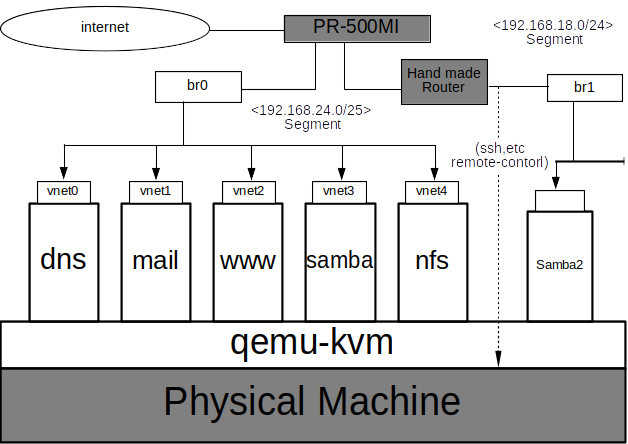
\includegraphics{image201803-kansai/external.png}
\caption{$B30ItMQ%M%C%H%o!<%/$N?^(B}
\end{figure*}
\clearpage

\subsubsection{$B30ItMQ%M%C%H%o!<%/$N@_Dj(B}
$B30ItMQ$N%M%C%H%o!<%/$G$N3F(BVM$B$N%M%C%H%o!<%/%G%P%$%9$N@_Dj$O!"Bh0l$K(Bvirt-manager$B$r;H$$2>A[%M%C%H%o!<%/$r@\B3$9$k2>A[(Bbridge$B$r:n@.$7$^$9!#<!$K(BVM$B$N%M%C%H%o!<%/%$%s%?!<%U%'%$%9$O!"(Bqemu$B$G%(%_%e%l!<%H$5$l$k(BTAP$B%G%P%$%9$r:n@.$7$F!"C1=c$KF~=PNO$r@\B3$9$k!V(Btap$B!W$r:n$j$^$9!#$3$N(Btap$B$O5<;wE*$J(Bethernet$B%G%P%$%9$G(BLinux$B%+!<%M%k$N5!G=$G$9!#$3$N2>A[E*$J(Bethernet$B%G%P%$%9$r!"F1$8$/(BLinux$B$N%+%M!<%k$N5!G=$G$"$k2>A[(Bbridge$B$G@\B3$9$k$3$G!"(BVM$B$O<B%G%P%$%9$d$[$+$N(BVM$B$H@\B3$9$k$3$H$,$G$-$^$9!#(B

$B$?$@$7!"(Bvirt-manager$B$G:n@.$9$k2>A[(Bbridge$B$O(Bdefault$B$G%5%V%M%C%H$r@_Dj$G$-$^$;$s!#$J$N$G!"(Binterfaces$B%U%!%$%k$rD>@\!"JT=8$7$F%5%V%M%C%H$r@_Dj$7$^$9!#$^$?!"(BHand made Router$B!"(BVM$B$N(BDNS$B$NN>J}$K(Bbind$B%Q%C%1!<%8$r%$%s%9%H!<%k$7!"30ItMQ%M%C%H%o!<%/$r9=C[$7$^$9!#(B

$B<!$K!"(BHand made Router$B$O%k!<%?$K$9$k$?$a$K!"(Biptables$B$H(Biptables-persisten$B$N%Q%C%1!<%8$r;H$$$^$9!#$^$?!"(B/etc/sysctl.conf$B$N(Bnet.ipv4.ip$B!2(Bforward=1$B$N%3%a%s%H$r30$7$F$*$-$^$9!#6qBNE*$K$O(B

\begin{itemize}
\item $B2>A[(Bbridge$B!"(BHand made Router$B$G$N%5%V%M%C%H$N@_Dj(B\\
VM$B$rAv$i$;$k<B5!$O(B qemu-kvm virt-manager$B$r%$%s%9%H!<%k$7$F@_Dj$7$^$9!#$=$7$FF15!$N(B/etc/network/interfaces$B$r0J2<$N$h$&$KD>@\!"JT=8$7$^$9!#(B
\begin{commandline}
# The loopback network interface
auto lo
iface lo inet loopback

# The primary network interface
allow-hotplug br0
iface br0 inet static
   address 192.168.24.108
   netmask 255.255.255.128
   gateway 192.168.24.1
   bridge$B!2(Bports enp9s0
   bridge$B!2(Bstp on
   bridge$B!2(Bfd 0.0
# This is an autoconfigured IPv6 interface
iface enp9s0 inet6 auto

# The secondary network interface
auto enx0022cf56e5ca
allow-hotplug enx0022cf56e5ca
iface enx0022cf56e5ca inet static
address 192.168.18.80
netmask 255.255.255.0
gateway 192.168.18.80
# This is an autoconfigured IPv6 interface
iface enx0022cf56e5ca inet6 auto
\end{commandline}
$B<!$K(BHand made Router$B$O%k!<%?$H$7$F5!G=$7!"(BVM$B$N%b%K%?!<$HJ]<i$b9T$$!"%$%s%?!<%M%C%H$+$i$NF~8}$K$b$7$^$9!#@_Dj$H$7$F$O(B /etc/network/interfaces$B$H(B/etc/iptables/rules.v4$B$r0J2<$NMM$K$7$^$9!#(B\\
--------interfaces--------
\begin{commandline}
# The loopback network interface
auto lo
iface lo inet loopback

# The primary network interface
auto enp2s1
allow-hotplug enp2s1
iface enp2s1 inet static
address 192.168.24.88
netmask 255.255.255.128
gateway 192.168.24.1

# This is an autoconfigured IPv6 interface
iface enp2s1 inet6 auto

# The secondary network interface
allow-hotplug ens32
iface ens32 inet static
address 192.168.18.1
netmask 255.255.255.0
gateway 192.168.18.1

# This is an autoconfigured IPv6 interface
iface ens32 inet6 auto
\end{commandline}
\clearpage
--------rules.v4--------
\begin{commandline}
# Generated by iptables-save v1.6.0 on Sat Nov 18 17:30:00 2017
*filter
:INPUT ACCEPT [0:0]
:FORWARD ACCEPT [0:0]
:OUTPUT ACCEPT [0:0]

-A INPUT -i lo -j ACCEPT
...(Omltted)...
-A INPUT -i enp2s1 -m state --state RELATED,ESTABLISHED -j ACCEPT
-A INPUT -i enp2s1 -j DROP
...(Omltted)...
-A FORWARD -o ens32 -j REJECT --reject-with icmp-port-unreachable
-A FORWARD -i enp2s1 -m state --state RELATED,ESTABLISHED -j ACCEPT
-A FORWARD -o ens32 -m state --state NEW,ESTABLISHED -j ACCEPT

-A FORWARD -i enp2s1 -j DROP
-A FORWARD -o ens32 -j DROP

-A OUTPUT -o lo -j ACCEPT
...(Omltted)...
-A OUTPUT -o ens32 -m state --state NEW,ESTABLISHED -j ACCEPT
-A OUTPUT -o ens32 -j DROP
COMMIT
# Completed on Sat Mar 25 17:12:38 2017

# Generated by iptables-save v1.6.0 on Sat Apr 29 10:00:07 2017
*mangle
:PREROUTING ACCEPT [0:0]
:INPUT ACCEPT [0:0]
:FORWARD ACCEPT [0:0]
:OUTPUT ACCEPT [0:0]
:POSTROUTING ACCEPT [0:0]
-A POSTROUTING -o ens32 -p udp -m udp --dport 68 -j CHECKSUM --checksum-fill
COMMIT
# Completed on Sat Aug 26 16:07:34 2017

# Generated by iptables-save v1.4.21 on Sat Aug 26 16:07:34 2017
*nat
:PREROUTING ACCEPT [0:0]
:INPUT ACCEPT [0:0]
:OUTPUT ACCEPT [0:0]
:POSTROUTING ACCEPT [0:0]

-A POSTROUTING -s 192.168.18.0/24 ! -d 192.168.18.0/24 -j SNAT --to-source 192.168.24.88
COMMIT
# Completed on Sat Nov 18 17:30:00 2017  
\end{commandline}

\clearpage

\item bind$B$N3F%9%F!<%?%9$r;H$C$?30ItMQ%M%C%H%o!<%/$N@_Dj(B\\
$B!!(BVM$B$N(BDNS$B!"(BHand Made Router$B$K%$%s%9%H!<%k$9$k(Bbind$B%Q%C%1!<%8$N(Bnamed.conf$B$N@_DjJ}K!$O2<?^$NDL$j!#35MW$H$7$F$O@_Dj%U%!%$%k$N(Bnamed.conf$B$K(Binclude$B%9%F!<%a%s%H$r;H$$!"(Bacl$B%9%F!<%H%a%s%H!"(Boptions$B%9%F!<%H%a%s%H$N@_Dj%U%!%$%k$rA^F~$7$^$9!#F1MM$K(Bview$B%9%F!<%H%a%s%H$G!">r7oIU$1%U%!%$%k$K$h$kF0:n$rDj5A$7!"(Binclude$B%9%F!<%H%a%s%H$G>r7o%U%!%$%k$rA^F~$7$^$9!#(B
%$B?^7A$NA^F~(B
\begin{figure*}[!h]
\centering
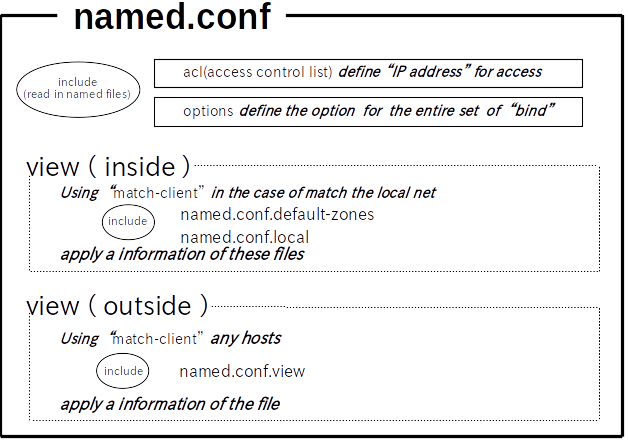
\includegraphics{image201803-kansai/named_conf.png}
\caption{named.conf$B$N?^(B}
\end{figure*}

$B0J2<!"3F@_Dj%U%!%$%k$N>\:Y$G$9!#(B
\clearpage

\item named.conf$B!J(Bbind$B$N@_Dj%U%!%$%k!K(B
\begin{commandline}
// This is the primary configuration file for the BIND DNS server named.
//
// Please read /usr/share/doc/bind9/README.Debian.gz for information on the 
// structure of BIND configuration files in Debian, *BEFORE* you customize 
// this configuration file.
//
// If you are just adding zones, please do that in /etc/bind/named.conf.local

include "/etc/bind/named.conf.acl";
include "/etc/bind/named.conf.options";

view "internal"{
	match-clients { localnet; };
	recursion yes;

include "/etc/bind/named.conf.local";
include "/etc/bind/named.conf.default-zones";

};

view "external" {
	match-clients { any; };
	recursion no;

include "/etc/bind/named.conf.view";

};    
\end{commandline}
$B3F%9%F!<%H%a%s%H$4$H$N@_Dj%U%!%$%k$O0J2<$N$h$&$K$J$j$^$9!#(B\\

\item acl$B%9%F!<%H%a%s%H!J%"%/%;%9$9$k%M%C%H%o!<%/$N(BIP$B%"%I%l%9$N@_Dj%U%!%$%k!K(B
\begin{commandline}
acl localnet{ 
	192.168.24.0/25;
	192.168.24.128/26;
	192.168.24.192/26;
	192.168.18.0/24; 
	127.0.0.1; 
};
\end{commandline}

\item options$B%9%F!<%H%a%s%H!J%*%W%7%g%s$G(Bbind$BA4BN$NF0:n$r@_Dj$9$k!K(B
\begin{commandline}
options {
	directory "/var/cache/bind";

	// If there is a firewall between you and nameservers you want
	// to talk to, you may need to fix the firewall to allow multiple
	// ports to talk.  See http://www.kb.cert.org/vuls/id/800113

	// If your ISP provided one or more IP addresses for stable 
	// nameservers, you probably want to use them as forwarders.  
	// Uncomment the following block, and insert the addresses replacing 
	// the all-0's placeholder.

	forwarders {
	 	8.8.8.8; 8.8.4.4;
	};

	//========================================================================
	// If BIND logs error messages about the root key being expired,
	// you will need to update your keys.  See https://www.isc.org/bind-keys
	//========================================================================
	dnssec-validation auto;
	allow-query { any; };
        allow-transfer{ 
		localnet;
		8.8.8.8;
		8.8.4.4; 
	};
	version "no version";
	auth-nxdomain no;    # conform to RFC1035
	listen-on-v6 { any; };
};
\end{commandline}
\clearpage

\item viwe$B%9%F!<%H%a%s%H!JFbIt!K(B\\
  match-client$B$r;H$$%m!<%+%k%M%C%H$K0J2<$N@_Dj%U%!%$%k$rE,MQ$9$k!#(B\\
--- named.conf.default-zone ---
\begin{commandline}
// prime the server with knowledge of the root servers
zone "." {
	type hint;
	file "/etc/bind/db.root";
};

// be authoritative for the localhost forward and reverse zones, and for
// broadcast zones as per RFC 1912

zone "localhost" {
	type master;
	file "/etc/bind/db.local";
};

zone "127.in-addr.arpa" {
	type master;
	file "/etc/bind/db.127";
};

zone "0.in-addr.arpa" {
	type master;
	file "/etc/bind/db.0";
};

zone "255.in-addr.arpa" {
	type master;
	file "/etc/bind/db.255";
};
\end{commandline}
zone$B%9%F!<%H%a%s%H!J%[%9%HL>$H(BIP$B%"%I%l%9$NBP1~4X78$N%j%9%H$rDj5A$9$k!K$G;H$o$l$F$$$k$3$l$i$N%U%!%$%k$O(Bdefault$B$G(Bbind$B%U%)%k%@$K4^$^$l$F$$$^$9!#(B\\
--- named.conf.local ---
\begin{commandline}
//
// Do any local configuration here
//
zone "kinsen.gr.jp" {
	type master;
	file "/etc/bind/db.in-kinsen.gr.jp";
};
zone "24.168.192.in-addr.arpa" {
	type master;
	file "/etc/bind/db.192.168.24";
};
zone "18.168.192.in-addr.arpa" {
	type master;
	file "/etc/bind/db.192.168.18";
};
// Consider adding the 1918 zones here, if they are not used in your
// organization
//include "/etc/bind/zones.rfc1918";
\end{commandline}
$B0J>e$N%U%!%$%k$O0J2<$NDL$j$G$9!#(B
\clearpage

--- db.in-kinsen.gr.jp ---
\begin{commandline}
;
; BIND data file for kinsen.gr.jp
;
$TTL	86400
@	IN     SOA      bandai.kinsen.gr.jp. root.bandai.kinsen.gr.jp. (
		              1         ; Serial
			   1800         ; Refresh
			    900         ; Retry
			 604800         ; Expire
			   1200 )       ; Negative Cache TTL

		IN      NS      dns

; localhost
localhost       IN      A       127.0.0.1
localhost       IN      AAAA    ::1

; Mail exchange
                IN      MX      0 mail.kinsen.gr.jp.
;
; Host entry
;
mizu0           IN      A       192.168.18.1
;               IN      AAAA    2001
mizu1           IN      A       192.168.18.2
;               IN      AAAA    2001
kamaba          IN      A       192.168.18.80
;               IN      AAAA    2001
noren           IN      A       192.168.24.108
;               IN      AAAA    2001
dns             IN      A       192.168.24.81
;               IN      AAAA    2001:
mail            IN      A       192.168.24.82
;               IN      AAAA    2001:
www             IN      A       192.168.24.83
;               IN      AAAA    2001:
karan           IN      A       192.168.24.84
;               IN      AAAA    2001:
datuiba         IN      A       192.168.24.85
;               IN      AAAA    2001:
bandai          IN      A       192.168.24.88
;               IN      AAAA    2001:
yubune          IN      A       192.168.24.18
;               IN      AAAA    2001:
;
; Alias
;www            IN      CNAME    noren
;
; Domain
@               IN      A       192.168.24.88
                IN      MX 0    mail
\end{commandline}
--- db.192.168.24 ---
\begin{commandline}
;
; BIND data file for 192.168.24 network
;
$TTL	86400
@         IN    SOA     bandai.kinsen.gr.jp. root.bandai.kinsen.gr.jp. (
		              1         ; Serial
			   1800         ; Refresh
			    900         ; Retry
			 604800         ; Expire
			   1200 )       ; Negative Cache TTL

                IN      NS      dns
;
; Host entry
;
108             IN      PTR     noren.kinsen.gr.jp.
81              IN      PTR     dns.kinsen.gr.jp.
82              IN      PTR     mail.kinsen.gr.jp.
83              IN      PTR     www.kinsen.gr.jp.
84              IN      PTR     karan.kinsen.gr.jp.
85              IN      PTR     datuiba.kinsen.gr.jp.
88              IN      PTR     bandai.kinsen.gr.jp.
18              IN      PTR     yubune.kinsen.gr.jp.
\end{commandline}
\clearpage

\item view$B%9%F!<%H%a%s%H(B($B30It(B)\\
  match-client$B$r;H$$$9$Y$F$N30It(Bhost$B$K(Bnamed.conf.view$B%U%!%$%k$rE,MQ$9$k!#(B\\
--- named.conf.view ---
\begin{commandline}
zone "." {
	type hint;
	file "/etc/bind/db.root";
};
zone "kinsen.gr.jp"{
	type master;
	file "/etc/bind/db.out-kinsen.gr.jp";
};
zone "158.141.203.in-addr.arpa"{
	type master;
	file "/etc/bind/db.203.141.158";
};    
\end{commandline}
db.root$B%U%!%$%k$O(Bdefault$B$G(Bbind$B%U%)%k%@$K$"$j$^$9!#(Bout-kinsen.gr.jp$B!"(Bdb.203.141.158$B$K$D$$$F$O0J2<$NDL$j!#(B\\
--- out-kinsen.gr.jp ---
\begin{commandline}
;
; BIND data file for kinsen.gr.jp
;
$TTL	86400
@        IN      SOA    bandai.kinsen.gr.jp. root.bandai.kinsen.gr.jp. (
                              1         ; Serial
			   1800         ; Refresh
			    900         ; Retry
			 604800         ; Expire
			   1200 )       ; Negative Cache TTL
                         $B!!!!!!!!!!!!!!!!!!!!(B
                IN$B!!!!!!(BNS       dns

; localhost
localhost       IN      A       127.0.0.1
localhost       IN      AAAA    ::1

; Mail exchange
                IN      MX      0 mail.kinsen.gr.jp.
;
; Host entry
;
noren           IN      A       203.141.158.41
;               IN      AAAA    2001:
dns             IN      A       203.141.158.41
;               IN      AAAA    2001:
mail            IN      A       203.141.158.41
;               IN      AAAA    2001:
www             IN      A       203.141.158.41
;               IN      AAAA    2001:
karan           IN      A       203.141.158.41
;               IN      AAAA    2001:
datuiba         IN      A       203.141.158.41
;               IN      AAAA    2001:
bandai          IN      A       203.141.158.41
;               IN      AAAA    2001:
yubune          IN      A       203.141.158.41
;               IN      AAAA    2001:
;
; Domain
@               IN      A       203.141.158.41
                IN      MX 0    mail
\end{commandline}
\clearpage

--- db.203.141.58 ---
\begin{commandline}
;
; BIND data file for 203.141.158 network
;
$TTL    86400
@       IN      SOA     bandai.kinsen.gr.jp. root.bandai.kinsen.gr.jp. (
                              1         ; Serial
                           1800         ; Refresh
                            900         ; Retry
                         604800         ; Expire
                           1200 )       ; Negative Cache TTL

                  IN        NS      dns
;
; Host entry
;
41		IN	PTR	noren.kinsen.gr.jp.
41		IN	PTR	dns.kinsen.gr.jp.
41		IN	PTR	mail.kinsen.gr.jp.
41		IN	PTR	www.kinsen.gr.jp.
41		IN	PTR	karan.kinsen.gr.jp.
41		IN	PTR	datuiba.kinsen.gr.jp.
41		IN	PTR	bandai.kinsen.gr.jp.
41		IN	PTR	yubune.kinsen.gr.jp.
\end{commandline}
\end{itemize}

\subsection{$BFbItMQ%M%C%H%o!<%/(B}
\subsubsection{$BFbItMQ%M%C%H%o!<%/$N35MW(B}
$BFbItMQ%M%C%H%o!<%/$O<B5!(BPC$B$K2>A[%k!<%?$r:n$j!"(BWifi$B7PM3$G<B5!>e$GAv$k(BVM$B$r%W%i%$%Y!<%H%M%C%H$r(B3$B$KJ,$1$?$=$l$>$l$N%;%0%a%s%H!J(B192.168.24.0/25 192.168.24.128/26 1923168.24.192/26$B!K$K$D$J$.$^$9!#(B\\
$B35MW$O2<?^$NDL$j!#(B

%$B?^7A$NA^F~(B
\begin{figure*}[!h]
\centering
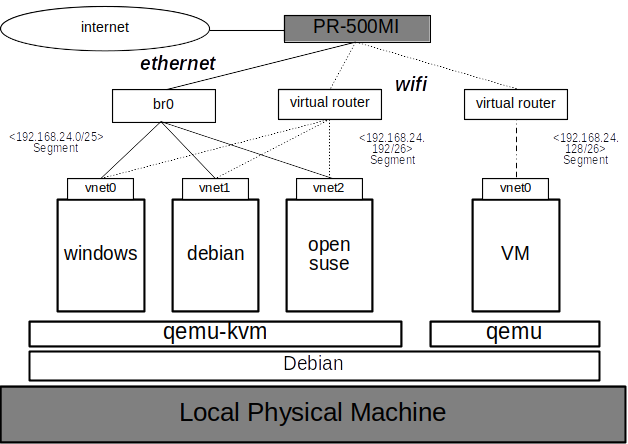
\includegraphics{image201803-kansai/internal.png}
\caption{$BFbItMQ%M%C%H%o!<%/$N?^(B}
\end{figure*}
\clearpage

\subsubsection{$BFbItMQ%M%C%H%o!<%/$N@_Dj(B}
$BFbItMQ%M%C%H%o!<%/$N@_Dj$O!"A0Ds$H$7$F(Bvirt-manager$B$N(BConnection Details$B$N(Bvirtual network$B$G2>A[%k!<%?$r:n$C$F$*$-$^$9!#$^$?!"<B5!(BPC$B$r%k!<%?$K$9$k;v$rA0Ds$K$7$F$$$^$9$N$G!"A0=R$N(BHand made Router$B$N$h$&$K!"(Binterfaces$B$H(Brules.v4$B$N%U%!%$%k$r0J2<$N$h$&$K@_Dj$7$^$9!#(B

--- interfaces ---
\begin{commandline}
# This file describes the network interfaces available on your system
# and how to activate them. For more information, see interfaces(5).

source /etc/network/interfaces.d/*

# The loopback network interface
auto lo
iface lo inet loopback

# The primary network interface
allow-hotplug wlp1s0
iface  wlp1s0 inet dhcp

# This is an autoconfigured IPv6 interface
iface wlp1s0 inet6 auto

# The primary network interface
allow-hotplug enx0022cf56e5ca
iface br0 inet static
   address 192.168.24.8
   netmask 255.255.255.128
   gateway 192.168.24.1
   bridge_ports enx0022cf56e5ca
   bridge_stp on
   bridge_fd 0.0
# This is an autoconfigured IPv6 interface
iface enx0022cf56e5ca inet6 auto
iface br0 inet6 auto
\end{commandline}
\clearpage

--- rules.v4 ---
\begin{commandline}
# Generated by iptables-save v1.6.0 on Sat Apr 29 10:00:07 2017
*filter
:INPUT ACCEPT [0:0]
:FORWARD ACCEPT [0:0]
:OUTPUT ACCEPT [0:0]
-A INPUT -i lo -j ACCEPT
-A INPUT -i enx0022cf56e5ca -j ACCEPT
-A INPUT -i br0 -j ACCEPT

-A INPUT -i wlp1s0 -p udp -m udp --dport 123 -j ACCEPT
-A INPUT -i wlp1s0 -p udp -m udp --dport 53 -j ACCEPT
-A INPUT -i wlp1s0 -p tcp -m tcp --dport 53 -j ACCEPT
-A INPUT -i wlp1s0 -p udp -m udp --dport 67:68 -j ACCEPT
-A INPUT -i wlp1s0 -p tcp -m tcp --dport 80 -j ACCEPT
-A INPUT -i wlp1s0 -p tcp -m tcp --dport 443 -j ACCEPT
-A INPUT -i wlp1s0 -p udp -m udp --dport 111 -j ACCEPT
-A INPUT -i wlp1s0 -p tcp -m tcp --dport 111 -j ACCEPT
-A INPUT -i wlp1s0 -p udp -m udp --dport 2049 -j ACCEPT
-A INPUT -i wlp1s0 -p tcp -m tcp --dport 2049 -j ACCEPT
-A INPUT -i wlp1s0 -p udp -m udp --dport 445 -j ACCEPT
-A INPUT -i wlp1s0 -p tcp -m tcp --dport 445 -j ACCEPT
-A INPUT -i wlp1s0 -p tcp -m tcp --dport 5900:6000 -j ACCEPT
-A INPUT -i wlp1s0 -p udp -m udp --dport 32800:32805 -j ACCEPT
-A INPUT -i wlp1s0 -p tcp -m tcp --dport 32800:32805 -j ACCEPT
-A INPUT -i wlp1s0 -m state --state RELATED,ESTABLISHED -j ACCEPT
-A INPUT -i wlp1s0 -j DROP


-A FORWARD -i wlp1s0 -p udp -m udp --dport 123 -j ACCEPT
-A FORWARD -o virbr1 -p udp -m udp --sport 123 -m state --state ESTABLISHED -j ACCEPT
-A FORWARD -i wlp1s0 -p udp -m udp --dport 53 -j ACCEPT
-A FORWARD -o virbr1 -p udp -m udp --sport 53 -m state --state ESTABLISHED -j ACCEPT
-A FORWARD -i wlp1s0 -p tcp -m tcp --dport 53 -j ACCEPT
-A FORWARD -o virbr1 -p tcp -m tcp --sport 53 -m state --state ESTABLISHED -j ACCEPT
-A FORWARD -i wlp1s0 -p udp -m udp --dport 67 -j ACCEPT
-A FORWARD -o virbr1 -p udp -m udp --sport 67 -m state --state ESTABLISHED -j ACCEPT
-A FORWARD -i wlp1s0 -p udp -m udp --dport 68 -j ACCEPT
-A FORWARD -o virbr1 -p udp -m udp --sport 68 -m state --state ESTABLISHED -j ACCEPT
-A FORWARD -i wlp1s0 -p tcp -m tcp --dport 80 -j ACCEPT
-A FORWARD -o virbr1 -p tcp -m tcp --sport 80 -m state --state ESTABLISHED -j ACCEPT
-A FORWARD -i wlp1s0 -p tcp -m tcp --dport 443 -j ACCEPT
-A FORWARD -o virbr1 -p tcp -m tcp --sport 443 -m state --state ESTABLISHED -j ACCEPT
-A FORWARD -i wlp1s0 -p udp -m udp --dport 445 -j ACCEPT
-A FORWARD -o virbr1 -p udp -m udp --sport 445 -m state --state ESTABLISHED -j ACCEPT
-A FORWARD -i wlp1s0 -p tcp -m tcp --dport 445 -j ACCEPT
-A FORWARD -o virbr1 -p tcp -m tcp --sport 445 -m state --state ESTABLISHED -j ACCEPT
-A FORWARD -i wlp1s0 -p tcp -m tcp --dport 5900:6000 -j ACCEPT
-A FORWARD -o virbr1 -p tcp -m tcp --sport 5900:6000 -m state --state ESTABLISHED -j ACCEPT
-A FORWARD -o virbr1 -j REJECT --reject-with icmp-port-unreachable
-A FORWARD -i wlp1s0 -m state --state RELATED,ESTABLISHED -j ACCEPT
-A FORWARD -o virbr1 -m state --state NEW,ESTABLISHED -j ACCEPT
-A FORWARD -i wlp1s0 -j DROP
-A FORWARD -o virbr1 -j DROP

-A OUTPUT -o lo -j ACCEPT
-A OUTPUT -o br0 -j ACCEPT

-A OUTPUT -o virbr1 -p udp -m udp --sport 123 -j ACCEPT
-A OUTPUT -o virbr1 -p udp -m udp --sport 53 -j ACCEPT
-A OUTPUT -o virbr1 -p tcp -m tcp --sport 53 -j ACCEPT
-A OUTPUT -o virbr1 -p udp -m udp --sport 67:68 -j ACCEPT
-A OUTPUT -o virbr1 -p tcp -m tcp --sport 80 -j ACCEPT
-A OUTPUT -o virbr1 -p tcp -m tcp --sport 443 -j ACCEPT
-A OUTPUT -o virbr1 -p udp -m udp --sport 111 -j ACCEPT
-A OUTPUT -o virbr1 -p tcp -m tcp --sport 111 -j ACCEPT
-A OUTPUT -o virbr1 -p udp -m udp --sport 2049 -j ACCEPT
-A OUTPUT -o virbr1 -p tcp -m tcp --sport 2049 -j ACCEPT
-A OUTPUT -o virbr1 -p udp -m udp --sport 445 -j ACCEPT
-A OUTPUT -o virbr1 -p tcp -m tcp --sport 445 -j ACCEPT
-A OUTPUT -o virbr1 -p tcp -m tcp --sport 5900:6000 -j ACCEPT
-A OUTPUT -o virbr1 -p udp -m udp --sport 32800:32805 -j ACCEPT
-A OUTPUT -o virbr1 -p tcp -m tcp --sport 32800:32805 -j ACCEPT
-A OUTPUT -o virbr1 -m state --state NEW,ESTABLISHED -j ACCEPT
-A OUTPUT -o virbr1 -j DROP
COMMIT

*mangle
:PREROUTING ACCEPT [0:0]
:INPUT ACCEPT [0:0]
:FORWARD ACCEPT [0:0]
:OUTPUT ACCEPT [0:0]
:POSTROUTING ACCEPT [0:0]
-A POSTROUTING -o virbr1 -p udp -m udp --dport 68 -j CHECKSUM --checksum-fill
COMMIT

*nat
:PREROUTING ACCEPT [0:0]
:INPUT ACCEPT [0:0]
:OUTPUT ACCEPT [0:0]
:POSTROUTING ACCEPT [0:0]
-A POSTROUTING -s 192.168.1.128/26 ! -d 192.168.1.128/26 -j MASQUERADE
-A POSTROUTING -s 192.168.1.192/26 ! -d 192.168.1.192/26 -j MASQUERADE
COMMIT
# Completed on Sat Jul 22 20:16:41 2017
\end{commandline}

\subsection{$B$^$H$a(B}
$B0J>e$,!"!V2f$,2H$N2>A[%M%C%H%o!<%/!W$NFbMF$G$9!#$?$@!"<B:]$N$H$3$mK\Mh$N%7%s%/%i%$%"%s%H$NL\E*$+$i$O%:%l$F$$$^$9!#:#8e$O(Bv6$B$N$X$NBP1~$d!"(BOS$B%5!<%P$J$k$b$NMQ0U$7$F!"99$J$k!IMxJX@-!I$rDI5a$9$k$D$b$j$G$9!#(B

%201803 tokyo
\dancersection{go / debian $B$G$N5!3#3X=,4D6-9=C[$K$D$$$F(B}{ysaito}
%-------------------------------------------------------------------------------

\subsection{$B$O$8$a$K(B}
$B5!3#3X=,$H$$$&J,Ln$G$O(B, python, $B$"$k$$$O(B, R $B$,?M5$$rFsJ,$9$k(B.
$B$7$+$7(B, $BBh;0$NA*Br;h$H$7$F(B, Go $B$K$h$k5!3#3X=,4D6-$,$"$k(B.
Go $B$G5!3#3X=,$r9T$&%a%j%C%H$O(B, $B@EE*7?0BA4$d(B, goroutine, channel, $B$J$I$NJB9T=hM}$N%a%j%C%H$,$"$k$,(B, $B:G$bCmL\$9$Y$-E@$O(B, $B%$%s%U%i(B, $B%7%9%F%`%W%m%0%i%_%s%0$KBP$9$k?FOB@-$G$"$k$H9M$($k(B.

$B:#2s$O(B, $B5!3#3X=,$=$N$b$N$N2r@b$K$OF'$_9~$^$:(B, Go/Debian $B$K$h$k5!3#3X=,4D6-$N9=C[$K?($l$?$$(B.

$B4D6-$O(B debian 9.4 (stretch) $B$rMxMQ$9$k(B.

\subsection{$B=q@R$N>R2p(B}
Machine Learning With Go (Packt publishing)

\url{https://www.packtpub.com/big-data-and-business-intelligence/machine-learning-go}

\subsection{kuberetes, docker $B$N=`Hw(B}
VM$B%5%]!<%H$O(B, $BM-8z$K$;$:%m!<%+%k$G$N<B9T$rA0Ds$H$7$F(B minikube $B$rF3F~$9$k(B.

docker $B%j%]%8%H%j$NF3F~(B
\begin{commandline}
apt install curl apt-transport-https ca-certificates software-properties-common
curl -fsSL https://download.docker.com/linux/debian/gpg | sudo apt-key add -
\end{commandline}

fingerprint $B$N3NG'(B
\begin{commandline}
apt-key fingerprint 0EBFCD88

pub   rsa4096 2017-02-22 [SCEA]
      9DC8 5822 9FC7 DD38 854A  E2D8 8D81 803C 0EBF CD88
uid           [ unknown] Docker Release (CE deb) <docker@docker.com>
sub   4096R/F273FCD8 2017-02-22 [S]
\end{commandline}

docker $B$NF3F~(B
\begin{commandline}
apt install docker-ce
docker version
Docker version 18.03.0-ce, build 0520e24

# $BF~NO%G!<%?$r=hM}$9$k%"%k%4%j%:%`$,$N$C$?(B docker image $B$rF3F~$9$k(B
docker pull dwhitena/goregtrain:single
\end{commandline}


minikube, kubectl $B$NF3F~(B
\begin{commandline}
curl -Lo minikube https://storage.googleapis.com/minikube/releases/latest/minikube-linux-amd64 && \
chmod +x minikube && sudo mv minikube /usr/local/bin/
curl -Lo kubectl \
https://storage.googleapis.com/kubernetes-relesase/release/\
$(curl -s https://storage.googleapis.com/kubernetes-release/release/stable.txt)/bin/linux/amd64/kubectl && \
chmod +x kubectl && mv kubectl /usr/local/bin/

minikube version
minikube version v0.25.2

kubectl version
Client Version: version.Info{Major:"1", Minor:"9", GitVersion:"v1.9.6",
GitCommit:"9f8ebd171479bec0ada837d7ee641dec2f8c6dd1", GitTreeState:"clean",
BuildDate:"2018-03-21T15:21:50Z", GoVersion:"go1.9.3", Compiler:"gc",
Platform:"linux/amd64"}
\end{commandline}

minikube $BMQ$N@_Dj$H(B minikube $B$N3+;O(B
\begin{commandline}
export MINIKUBE_WANTUPDATENOTIFICATION=false
export MINIKUBE_WANTREPORTERRORPROMPT=false
export MINIKUBE_HOME=$HOME
export CHANGE_MINIKUBE_NONE_USER=true
mkdir $HOME/.kube || true
touch $HOME/.kube/config

export KUBECONFIG=$HOME/.kube/config

minikube start --vm-driver=none

\end{commandline}

pachyderm $B$NF3F~(B
\begin{commandline}
curl -o /tmp/pachctl.deb -L \
https://github.com/pachyderm/pachyderm/releases/download/v1.7.0rc4/pachctl_1.7.0rc4_amd64.deb && \
sudo dpkg -i /tmp/pachctl.deb

pachctl deploy local
\end{commandline}

\subsection{pachyderm $B$H$O(B}
pachyderm$B$H$O(B, $B%G!<%?$N%P!<%8%g%s4IM}$d(B, $B5!3#3X=,$N=hM}$r%Q%$%W%i%$%s$G$D$J$0$3$H$,$G$-$k(B go $B@=$N%=%U%H%&%'%"$G$"$k(B.
$B>\$7$/$O(B, \url{https://pachyderm.io} $B$K$F>pJs$,$"$k(B.

\subsection{$B9=@.$9$k35MW(B}

diabetes.csv $B$+$i(B, go $B$K$h$k5!3#3X=,%"%k%4%j%:%`$K$h$j!"%b%G%k!J(Bcsv$B$+$iF@$i$l$?4X?t$N%Q%i%a!<%?!K$r@8@.$7(B, model.json
$B?75,$KF@$i$l$?F~NO(B, 1.json $B$+$iM=B,(B, 1.json $B$r=PNO$9$k(B

\begin{commandline}
     +-------------------------------------------------------------+
     |                                                             |
     |                                                             |
     |  +----------+    +----------+    +------------+             |
     |  |          |    |          |    |            |             |
     |  |  $B3X(B   $B=,(B |  $B!!(B| $B%b(B $B%G(B $B%k(B |    |  $B%b(B  $B%G(B  $B%k(B|             |
     |  |          |    |          |    |            |             |
+-----> |          +--> |          |--> |            |             |
     |  diabetes.csv    | ./goregtrain  | model.json |             |
     |  |          |    |          |    |            |             |
     |  +----------+    +----------+    +-----+------+             |
     |                                        |                    |
     |                  +----------+    +-----v------+  +--------+ |
     |                  |          |    |            |  |        | |
     |                  | attributes    | $BM=(B  $BB,(B     |  | $BM=(B  $BB,(B | |
 +--------------------> |          +--> |            +> |        | |
     |                  |          |    |            |  |        | |
     |                  | 1.json   |    | ./goregpredict| 1.json | |
     |                  +----------+    +------------+  +--------+ |
     |                                                             |
     +-------------------------------------------------------------+
\end{commandline}
     
\subsection{$BF~NO$K;HMQ$9$k%G!<%?(B}
\url{https://github.com/PacktPublishing/Machine-Learning-With-Go/tree/master/Chapter09/building_a_scalable_pipeline/example2}

\subsection{go $B$K$h$C$F(B pachyderm $B$X@\B3$7%j%]%8%H%j$r:n$k(B}
\begin{commandline}
// localhost $B>e$N(B Kubernetes $B%/%i%9%?$N(B pachyderm $B$X@\B3$9$k(B
// $B%G%U%)%k%H$N(B pachyderm $B$N%]!<%H(B 30650
c, err := client.NewFromAddress("0.0.0.0:30650")
if err != nil {
log.Fatal(err)
}
defer c.Close()
// $B3X=,MQ$N%j%]%8%H%j$r:n@.(B "training."
if err := c.CreateRepo("training"); err != nil {
log.Fatal(err)
}
// $BM=B,$NF~NOMQ$N%j%]%8%H%j$r:n@.$9$k(B "attributes."
if err := c.CreateRepo("attributes"); err != nil {
log.Fatal(err)
}
// $B#2$D$N%j%]%8%H%j$K(B sanity check $B$r$*$3$J$&(B
repos, err := c.ListRepo(nil)
if err != nil {
log.Fatal(err)
}
// $B%j%]%8%H%j$N?t$r3NG'$9$k(B
if len(repos) != 2 {
log.Fatal("Unexpected number of data repositories")
}
\end{commandline}

$B%3%s%Q%$%k$H<B9T(B
\begin{commandline}
go build
./create
pachctl list-repo
NAME CREATED SIZE
attributes 3 seconds ago 0B
training 3 seconds ago 0B
\end{commandline}

\subsection{attribute $B%j%]%8%H%j(B, training $B%j%]%8%H%j$X%G!<%?$r%;%C%H$9$k(B}

\begin{commandline}
// Pachyderm $B$X@\B3$9$k(B
c, err := client.NewFromAddress("0.0.0.0:30650")
if err != nil {
log.Fatal(err)
}
defer c.Close()
// "attributes" $B%G!<%?%j%]%8%H%j$K%G!<%?$r(B "master" $B%V%i%s%A$K%3%_%C%H$9$k=hM}$r;O$a$k(B
commit, err := c.StartCommit("attributes", "master")
if err != nil {
log.Fatal(err)
}
// attributes $B$KF~$l$k(B JSON $B$r3+$/(B
f, err := os.Open("1.json")
if err != nil {
log.Fatal(err)
}
// attributes $B$X%U%!%$%k$r%W%C%H$9$k(B
if _, err := c.PutFile("attributes", commit.ID, "1.json", f); err != nil {
log.Fatal(err)
}
// $B%3%_%C%H$r40N;$5$;$k(B.
if err := c.FinishCommit("attributes", commit.ID); err != nil {
log.Fatal(err)
}
// "training" $B%G!<%?%j%]%8%H%j$N(B "master" $B%V%i%s%A$X%G!<%?$r%3%_%C%H$9$k=hM}$r;O$a$k(B.
commit, err = c.StartCommit("training", "master")
if err != nil {
log.Fatal(err)
}
// $B3X=,MQ$N%G!<%?%;%C%H%U%!%$%k$r3+$/(B
f, err = os.Open("diabetes.csv")
if err != nil {
log.Fatal(err)
}
// training $B%G!<%?%;%C%H$r(B $B3X=,MQ%G!<%?%j%]%8%H%j$KE83+$9$k(B.
if _, err := c.PutFile("training", commit.ID, "diabetes.csv", f); err !=
nil {
log.Fatal(err)
}
// $B%3%_%C%H$r40N;$5$;$k(B.
if err := c.FinishCommit("training", commit.ID); err != nil {
log.Fatal(err)
}
\end{commandline}

$B%3%s%Q%$%k$7$F<B9T$9$k(B
\begin{commandline}
# $B>e5-$N%3!<%I$r%3%s%Q%$%k$9$k(B
go build
# $B<B9T(B
./a

# $B%j%]%8%H%j$rI=<($9$k(B
pachctl list-repo
NAME CREATED SIZE
training 13 minutes ago 73.74KiB
attributes 13 minutes ago 210B

# training $B%j%]%8%H%j$N(B master $B%V%i%s%A$N%U%!%$%k$rI=<($9$k(B
pachctl list-file training master
NAME TYPE SIZE
diabetes.csv file 73.74KiB

# attributes $B%j%]%8%H%j$N(B master $B%V%i%s%A$N%U%!%$%k$rI=<($9$k(B
pachctl list-file attributes master
NAME TYPE SIZE
1.json file 210B
\end{commandline}

\subsection{model $B%9%F!<%8$N(BJSON $B$r=`Hw$9$k(B}

\begin{commandline}
{
  "pipeline": {
    "name": "model"
  },
  "transform": {
    "image": "dwhitena/goregtrain:single",
    "cmd": [
      "/goregtrain",
      "-inDir=/pfs/training",
      "-outDir=/pfs/out"
    ]
  },
  "parallelism_spec": {
    "constant": "1"
  },
  "input": {
    "atom": {
      "repo": "training",
      "glob": "/"
    }
  }
}
\end{commandline}

\subsection{model $B%9%F!<%8$N(BJSON $B$r=`Hw$9$k(B}

1.Pachyderm $B%G!<%?%Q%$%W%i%$%s$,(B model $B$H$$$&L>A0$G$"$k$3$H$r65$($k(B
2.Pachyderm $B$X(B, $B%b%G%k:n@.$K;H$&%"%k%4%j%:%`$r65$($k(B, docker $B%$%a!<%8$K$J$C$F$$$k@~7A2s5"%b%G%k$r;HMQ$9$k(B( dwhitena/goregtrain:single ), 
3. $B$=$7$F(B, $B3X=,MQ%G!<%?%U%!%$%k$H$N%Q%$%W%i%$%s$r65$($k(B

\begin{commandline}
# $B%Q%$%W%i%$%s$N:n@.(B
pachctl create-pipeline -f model.json

# pods $B$N>uBV3NG'(B
kubectl get pods
NAME READY STATUS RESTARTS AGE
etcd-2142892294-38ptw 1/1 Running 0 2h
pachd-776177201-04l6w 1/1 Running 0 2h
pipeline-model-v1-p0lnf 2/2 Running 0 1m

# pachyderm $B>e$N(B job $B3NG'(B
pachctl list-job
ID OUTPUT COMMIT STARTED DURATION RESTART PROGRESS DL UL STATE
14f052ae-878d-44c9-a1f9-ab0cf6d45227 model/a2c7b7dfb44a40e79318c2de30c7a0c8
3 minutes ago Less than a second 0 1 + 0 / 1 73.74KiB 160B success

# $B%G!<%?%j%]%8%H%j$r3NG'(B
pachctl list-repo
NAME CREATED SIZE
model 3 minutes ago 160B
training About an hour ago 73.74KiB
attributes About an hour ago 210B

# model master $B%V%i%s%A$K$"$k%U%!%$%k$r3NG'(B
pachctl list-file model master
NAME TYPE SIZE k8s
model.json file 160B

# model.json $B$NCf?H$r3NG'$9$k(B
pachctl get-file model master model.json
{
  "intercept": 152.13348416289818,
  "coefficients": [
    {
      "name": "bmi",
      "coefficient": 949.4352603839862
    }
  ]
}
\end{commandline}


\subsection{$BM=B,MQ$N%Q%$%W%i%$%s$r@_Dj$77k2L$rF@$k(B}

\begin{commandline}
{
  "pipeline": {
    "name": "prediction"
  },
  "transform": {
    "image": "dwhitena/goregpredict",
    "cmd": [
      "/goregpredict",
      "-inModelDir=/pfs/model",
      "-inVarDir=/pfs/attributes",
      "-outDir=/pfs/out"
    ]
  },
  "parallelism_spec": {
    "constant": "1"
  },
  "input": {
    "cross": [
    {
      "atom": {
        "repo": "attributes",
        "glob": "/*"
      }
    },
      {
        "atom": {
          "repo": "model",
          "glob": "/"
        }
      }
    ]
  }
}
\end{commandline}

\begin{commandline}
# prediction.json $B$X$N%G!<%?%Q%$%W%i%$%s$r:n@.$9$k(B
pachctl create-pipeline -f prediction.json

# pachyderm $B>e$N(B job $B$N%j%9%H$r3NG'$9$k(B
pachctl list-job
ID OUTPUT COMMIT STARTED DURATION RESTART PROGRESS DL UL STATE
03f36398-89db-4de4-ad3d-7346d56883c0
prediction/5ce47c9e788d4893ae00c7ee6b1e8431 About a minute ago Less than a
second 0 1 + 0 / 1 370B 266B success
14f052ae-878d-44c9-a1f9-ab0cf6d45227 model/a2c7b7dfb44a40e79318c2de30c7a0c8
19 minutes ago Less than a second 0 1 + 0 / 1 73.74KiB 160B success

# $B%j%]%8%H%j$N3NG'$r$9$k(B
pachctl list-repo
NAME CREATED SIZE
prediction About a minute ago 266B
model 19 minutes ago 160B
training About an hour ago 73.74KiB
attributes About an hour ago 210B

# prediction $B%j%]%8%H%j$N(B master $B%V%i%s%A$NCf?H$r3NG'$9$k(B
pachctl list-file prediction master
NAME TYPE SIZE
1.json file 266B

# 1.json $B%U%!%$%k$NCf?H$r3NG'$9$k(B
pachctl get-file prediction master 1.json
\end{commandline}

%201804 kansai
%\dancersection{$B:G6a$N(BDebian$B%Q%C%1!<%8:n@.4D6-(B - git-buildpackage, sbuild, autopkgtest $B$rNc$K(B -($B;qNAL5$7(B)}{$B:4!9LZ(B $BMNJ?(B}

%201806 tokyo
%-------------------------------------------------------------------------------
\dancersection{salsa$B$HEl5~%(%j%"(Bdebian$BJY6/2q$N(BWeb/$B869F%7%9%F%`$N;EAH$_(B}{$B?yK\!!E5=<(B}
%-------------------------------------------------------------------------------

\subsection{$B$O$8$a$K(B}

$BEl5~%(%j%"(Bdebian$BJY6/2q$G$O!"JY6/2q$r1?1D$9$k$K$"$?$j(Bweb$B%5%$%H$HJY6/2q$NH/I=;qNA$G$"$k869F%G!<%?$H%9%i%$%I%G!<%?$r07$C$F$$$^$9!#$3$l$i$N%G!<%?$OJY6/2q$N5DO@$r?<$a$?$j5-O?$H$7$F=EMW$J;q;:$K$J$C$F$$$^$9!#(B


$BEl5~%(%j%"(BDebian$BJY6/2q$N;qNA$NJ]B8@h$r(B \url{salsa.debian.org} $B$X0\9T$7$?$?$a!";qNA$r=hM}$9$k;EAH$_$H(Bsalsa$B$X$N0\9T:n6H$K$D$$$FJs9p$7$^$9!#(B


\subsection{$BEl5~%(%j%"(BDebian$BJY6/2q$N%7%9%F%`(B}

$BEl5~%(%j%"(BDebian$BJY6/2q$G$O!"1?1D$r9T$&$K$"$?$j0J2<$N%7%9%F%`$rMxMQ$7$F$$$^$9!#(B

\begin{itemize}
  \item web$B%5%$%H!V(B\url{https://tokyodebian-team.pages.debian.net/}$B!W(B\footnote{$B%j%]%8%H%j$O!"(B\url{https://salsa.debian.org/tokyodebian-team/tokyodebian-team.pages.debian.net}}
  \item $BH/I=<T$N869F%G!<%?!"%9%i%$%I%G!<%?$r=hM}$9$k(Btex$B$N869F%7%9%F%`(B\footnote{$B%j%]%8%H%j$O!"(B\url{https://salsa.debian.org/tokyodebian-team/monthly-report}}
  \item $B;22C<T?=$79~$_$H$7$F30It%5!<%S%9!V(Bconnpass$B!W(B\footnote{\url{https://connpass.com/}}
  \item DebianJP$B$N%a!<%j%s%0%j%9%H!JJY6/2q$N9pCN!"AjCL!"<ALd$NAk8}!K(B
\end{itemize}


salsa$B$rMxMQ$7$F$$$k$N$O!"(Bweb$B%5%$%H$H869F%G!<%?$N%U%!%$%k4IM}$r9T$&I,MW$J=hM}$H$J$j$^$9!#(B


\subsection{salsa.debian.org}

\subsubsection{salsa$B$H$O(B}

salsa$B$H$O!"(BDebian$B%W%m%8%'%/%H$,(B \url{salsa.debian.org} $B$H$7$F1?MQ$7$F$$$k3+H/<T8~$1$N%W%m%8%'%/%H4IM}%5!<%P$G$9!#(Bgitlab$B$r%$%s%9%H!<%k$7$?%5!<%P$K$J$C$F$*$j!"8=Be$N(Bgit$B$r;H$C$?%o!<%/%U%m!<$d(BKubernetes(k8s)$B$HO"7H$7$F(BCI/CD$B$r<B9T$9$k5!G=$r;}$C$F$$$^$9!#(B 


\subsubsection{alioth$B$+$i(Bsalsa$B$X$N0\9T(B}

Debian$B%W%m%8%'%/%H$G$O(B2003$BG/$+$i(B \url{alioth.debian.org} $B$H$$$&%W%m%8%'%/%H4IM}%5!<%P$r1?MQ$7$F$$$^$7$?!#(Balioth$B$O(BFusionForge\footnote{\url{http://www.fusionforge.org}}$B$H$$$&(BOSS$B$N(Bweb$B%Y!<%9$J%W%m%8%'%/%H4IM}%D!<%k$r%5!<%S%9$9$k%[%9%H$G$"$j!"(Bweb$B%5!<%P!&(Bwiki$B!&%a!<%j%s%0%j%9%H!&(BCVS/SVN/GIT$B$N%j%]%8%H%j$r%5!<%S%9$7$F$$$^$7$?(B\footnote{https://wiki.debian.org/Alioth/FAQ\#FusionForge}$B!#(B


$B$7$+$7!"(BFusionForge$B$O(B2016$BG/(B12$B7n(B10$BF|$K(B fusionforge-6.0.5 $B$r%j%j!<%9$7$F$+$i3+H/$,BZ$k>u67$K$J$j$^$9!#(Balioth$B%5!<%P$O(BDebian 7 (wheezy)$B$K(BFusionForge$B$r%$%s%9%H!<%k$7$F1?MQ$7$F$$$^$7$?$,!"%"%W%j%1!<%7%g%s$N99?7$,;_$^$C$?$3$H$+$i(Balioth$B$r:#8e$I$&$7$F$$$/$+5DO@$,;O$^$j$^$7$?!#(B


2017$BG/(B8$B7n(B17$BF|$K(BAlioth Sprint 2017$B$r9T$$(B\footnote{https://wiki.debian.org/Sprints/2017/Alioth}$B!"(Bgitlab$B$r%Y!<%9$K$7$?(Balioth$B$N8e7Q%5!<%P$N%W%m%H%?%$%W$r<BAu$7(B\footnote{https://wiki.debian.org/Salsa}$B!"%5!<%PL>$r(B"salsa"$B$H8F>N$9$k$3$H$K$J$j$^$9!#(B


salsa$B$O(B2017$BG/(B12$B7n(B15$BF|$K%Y!<%?1?MQ$KF~$j(B\footnote{salsa.debian.org (git.debian.org replacement) going into beta \url{https://lists.debian.org/debian-devel-announce/2017/12/msg00003.html}}$B!"(B2018$BG/(B1$B7n(B27$BF|$K%Y!<%?1?MQ$r=*N;$7K\2TF/$r3+;O$7$^$7$?(B\footnote{salsa.debian.org updates (leaving beta) \url{https://lists.debian.org/debian-devel-announce/2018/01/msg00004.html}}$B!#(B


$B$=$7$F!"(B2018$BG/(B5$B7n(B31$BF|$N(BDebian 7 (wheezy) LTS$B$N=*N;$H$H$b$K(Balioth$B%5!<%P$O%5!<%S%9$r=*N;$7!"$=$N5!G=$r(Bsalsa$B$X0z$-7Q$.$^$7$?!#(B


\subsubsection{salsa$B$NMxMQ$N;EJ}(B}

\subsubsubsection{$B%I%-%e%a%s%H(B}

salsa$B$N%I%-%e%a%s%H$O0J2<$K$"$j$^$9!#(BDoc$B$N%Z!<%8$K%"%+%&%s%H$N%;%C%H%"%C%W$+$i%A!<%`$N:n@.$^$G$NN.$l$,=q$$$F$"$j$^$9!#$=$N$[$+!"(Bgitlab$B$N%I%-%e%a%s%H$r;2>H$/$@$5$$!#(B

\begin{itemize}
  \item \url{https://wiki.debian.org/Salsa/}
  \item \url{https://wiki.debian.org/Salsa/Doc}
  \item \url{https://docs.gitlab.com/}
\end{itemize}

\subsubsubsection{$B%"%+%&%s%H$NEPO?(B}

salsa$B$O(BDebian Developer$B$N%f!<%64IM}$r9T$&(BLDAP$B%5!<%P$HO"7H$7$F$$$^$9!#$=$N$?$a!"(BDebian Developer$B$NJ}$O(Bdebian.org$B$N%a!<%k%"%I%l%9$rMxMQ$7$F(Bsalsa$B$X%m%0%$%s$G$-$^$9!#(B


Debian Developer$B0J30$NJ}$O!"(B\url{https://signup.salsa.debian.org/} $B$N%Z!<%8$G(Bsalsa$B$N%2%9%H%"%+%&%s%H$r:n@.$G$-$^$9!#$3$N$H$-!"%f!<%6%"%+%&%s%HL>$O(B"-guest"$B$H$$$&J8;zNs$rKvHx$K4^$a$kL?L>5,B'$K$J$C$F$$$^$9!#(B


\subsubsubsection{$B%A!<%`$N:n@.(B}

gitlab $B$G$O$^$:!V%A!<%`!W$H$$$&%f!<%6$N%0%k!<%W$r$D$/$j!"%A!<%`$NG[2<$K%W%m%8%'%/%H72$r$D$/$k7A$K$J$C$F$$$^$9!#(B

\url{https://signup.salsa.debian.org/} $B$N%Z!<%8$G%A!<%`$r:n@.$G$-$^$9!#%A!<%`$N:n@.$O(BDebian Developer$B0J30$NJ}$G$b2DG=$G$9!#%A!<%`L>$O!"(B"-team"$B$H$$$&J8;zNs$rKvHx$K4^$a$kL?L>5,B'$K$J$C$F$$$^$9!#(B

$B%A!<%`$r:n@.$9$k$H!"Nc$($P(B \url{https://salsa.debian.org/tokyodebian-team} $B$N$h$&$J(BURL$B$G%A!<%`$N%Z!<%8$K%"%/%;%9$G$-$k$h$&$K$J$j$^$9!#(B

$B$J$*!"%A!<%`$r:n@.$7$?%f!<%6$O=i4|@_Dj$G%A!<%`$N(BOwner$B8"8B$r;}$A$^$9!#(B


\subsubsubsection{$B%A!<%`$X$N%a%s%P$N;22C(B}

salsa$B$KB8:_$9$k%f!<%6%"%+%&%s%H$r%A!<%`$KDI2C$9$k$3$H$G%W%m%8%'%/%H$N;22C<T$rA}$d$9$3$H$,$G$-$^$9!#%f!<%6$NDI2C$O!"%A!<%`$N(BOwner$B$^$?$O(BMaster$B$N8"8B$r;}$C$F$$$k%f!<%6$,A`:n$G$-$^$9!#(B

$B$J$*%f!<%68"8B$O(B \url{https://docs.gitlab.com/ee/user/permissions.html} $B$K0lMw$,$"$j!"(BOwner$B!"(BMaster\footnote{\url{https://docs.gitlab.com/ee/user/permissions.html}$B$N%^%K%e%"%k$G$O(BMaintainer$B$K$J$C$F$$$^$9$,!"(Bsalsa$B$G$O(BMaster$B$K$J$C$F$$$^$9!#(B}$B!"(BDeveloper$B!"(BReporter$B!"(BGuest$B$N8"8B$,$"$j$^$9!#(B

$B$^$?!"<+J,$,$H$"$k%A!<%`$X;22C$7$?$$>l9g$O!"(Bsalsa$B$X%m%0%$%s$7$?>uBV$G%A!<%`$N%H%C%W%Z!<%8$K$"$k!V%"%/%;%98"8B$r%j%/%(%9%H$9$k!W%\%?%s$r2!2<$7$F$/$@$5$$!#$9$k$H%A!<%`$X$NDI2C0MMj$,%A!<%`$N4IM}<T$XDLCN$5$l!"5v2D$5$l$l$P%A!<%`$N%a%s%P$KDI2C$5$l$^$9!#(B


\subsubsubsection{$B%W%m%8%'%/%H$N:n@.!J!a(Bgit$B%j%]%8%H%j$N:n@.!K(B}

$B%A!<%`$N%Z!<%8$N1&>e$K$"$k!V!\!W%^!<%/$NItJ,$r%/%j%C%/$9$k$HI=<($9$k%a%K%e!<$+$i%W%m%8%'%/%H$r:n@.$G$-$^$9!#(B

$B%W%m%8%'%/%H(B1$B$D$K$D$-(Bgit$B%j%]%8%H%j(B1$B$D$r;}$D$3$H$,$G$-$^$9!#$=$N$?$a!"J#?t$N(Bgit$B%j%]%8%H%j$G9=@.$9$k%W%m%8%'%/%H$N>l9g$O!"%A!<%`$,J#?t$N%W%m%8%'%/%H$r$b$D$h$&$K$9$k$3$H$G<B8=$G$-$^$9!#(B


\subsubsubsection{CI/CD}

gitlab$B$O(BCI$B!J(BContinuous Integration$B!K$d(BCD$B!J(BContinuous Delivery$B!K$N5!G=$rHw$($F$$$^$9!#(B


$B%f!<%6$,(Bgit$B%j%]%8%H%j$X(Bpush$B$7$?%?%$%_%s%0$d(Bwebhook\footnote{https://docs.gitlab.com/ee/user/project/integrations/webhooks.html}$B$H$$$&;EAH$_$rMxMQ$7$F(BCI/CD$B$N=hM}$r<B9T$G$-$^$9!#<g$K%f%K%C%H%F%9%H$N<+F0<B9T$d1?MQ%5!<%P$X%3%_%C%H$7$?%U%!%$%k$N<+F0G[Hw!"%A%c%C%H$X$NDLCN$J$I$N=hM}$r9T$&$3$H$,9M$($i$l$^$9!#(B


gitlab$B$N(BCI/CD$B=hM}$O!"(B"Runner"$B$H$$$&(BKubernetes(K8s)$B$N%$%s%9%?%s%9$X=hM}$r%j%/%(%9%H$9$k;EAH$_$K$J$C$F$$$^$9!#(BRunner$B$K$O!"(B3$B$D$N<oN`$,$"$j$^$9(B\footnote{https://docs.gitlab.com/ee/ci/runners/}$B!#(B

\begin{itemize}
\item Shared Runners\footnote{Runner$B$N%5!<%P$OITB-$7$F$$$k$?$a%9%]%s%5!<$rJg=8Cf$G$9!#(B\url{https://wiki.debian.org/Salsa/Doc\#Quick_start}}
  \begin{itemize}
  \item gitlab$B%5!<%P$NA4%A!<%`!"A4%W%m%8%'%/%H6&MQ$NHFMQ(BRunner$B!#(B
  \item Kubernetes$B$N%P!<%8%g%s$d%$%s%9%?%s%9$rLd$o$:<B9T$7$F$h$$>l9g$O$3$l$r;XDj$9$k!#(B
  \end{itemize}
\item Group Runners
  \begin{itemize}
  \item 1$B$D$N%A!<%`Fb$N%W%m%8%'%/%H72$N$_$G@jM-$7$FMxMQ$G$-$kHFMQ(BRunner$B!#(B
  \end{itemize}
\item Specific Runners
  \begin{itemize}
  \item 1$B$D$N%A!<%`Fb$N%W%m%8%'%/%H72$N$_$G@jM-$7$FMxMQ$G$-$k4D6-0MB88~$1(BRunner$B!#(B
  \item Runner$B$NF0:n4D6-$K1~$8$F(B1$B$D$^$?$OJ#?t$N%?%0$r@_Dj$9$k!#(B
  \item git$B%j%]%8%H%j$N(B".gitlab-ci.yml"$B$N(Btags$B%-!<$K%?%0$r;XDj$9$k$H!";XDj$7$?$9$Y$F$N%?%0$r$b$D(BSpecific Runner$B$X(BCI/CD$B=hM}$N<B9T$r%j%/%(%9%H$9$k!#(B
  \end{itemize}
\end{itemize}

gitlab$B$N(BCI/CD$B$O5!G=$d@_Dj9`L\$bB?$$$?$a!"(BGitLab$B$N%^%K%e%"%k(B\footnote{https://docs.gitlab.com/ee/ci/README.html}$B$r;2>H$7$F$/$@$5$$!#(B


\subsubsubsection{$B%f!<%68D?M%Z!<%8$N@_Dj(B}

$B%f!<%6$N8D?M@_Dj%Z!<%8$K$"$k!V(BSSH Keys$B!W%Z!<%8$+$i(BSSH$B80$rEPO?$9$k$3$H$,$G$-$^$9!#(B

SSH$B80$rEPO?$7$F$*$/$H!"(Bgit$B$N(Bpull$B$d(Bpush$B;~$NG'>Z$G%"%+%&%s%H$NF~NO$r$;$:$K:Q$`$?$a:n6H$,8zN(2=$9$k$G$7$g$&!#(B

salsa$B$N(Bgit$B%j%]%8%H%j$X(Bpull$B!"(Bpush$B$9$k%f!<%6$N%[%9%H$K$O!"0J2<$N(Bssh$B$N@\B3@_Dj$r$7$F$*$/$H$h$$$G$9!#(B

\begin{commandline}
$ cat ~/.ssh/config
Host salsa.debian.org
  User youraccount-guest
  IdentityFile ~/.ssh/id_rsa.yoursalsakey
\end{commandline}


\subsection{$BEl5~%(%j%"(BDebian$BJY6/2q$N(Bsalsa$B$N%7%9%F%`(B}

\subsubsection{alioth$B$+$i(Bsalsa$B$X$N0\9T$N@_7W$H:n6HFbMF(B}

$BEl5~%(%j%"(BDebian$BJY6/2q!J5Z$S4X@>(BDebian$BJY6/2q!K$G$O!"(B\url{alioth.debian.org} $B$K$"$k(Bgit$B%j%]%8%H%j5Z$S@EE*%U%!%$%k$N(Bweb$B8x3+5!G=$r;H$C$F$$$^$7$?!#(B

2018$BG/(B5$B7n$K(Balioth$B%5!<%P$,Dd;_$9$k$?$a!"(Bsalsa$B$X(Bgit$B%j%]%8%H%j$H(Bweb$B%5%$%H$r0\9T$9$k$h$&7W2h$7$^$7$?!#%7%9%F%`0\9T$N@_7W$H<B;\$9$k:n6H$O0J2<(BURL$B$K$^$H$a$F$$$^$9!#(B

\begin{itemize}
  \item \url{https://wiki.debian.org/tokyodebian_salsa_migrate}
\end{itemize}


\subsubsection{$B%U%!%$%k$N%i%$%;%s%9(B}

$BEl5~%(%j%"(BDebian$BJY6/2q$N(Bgit$B%j%]%8%H%j$K<}O?$7$F$$$k%U%!%$%k$O!"(Balioth$B$KG[CV$7$F$$$k;~Be$+$i%i%$%;%s%9$K(BGPLv2$B!J$^$?$O(BGPLv3$B!K$rE,MQ$9$k%k!<%k$H$7$F$$$^$9!#JY6/2q$K;22C$$$?$@$/J}$K$O%i%$%;%s%9$r$4M}2r$N>e!"%3%_%C%H$d%Q%C%A$NDs6!$r$*4j$$$$$?$7$^$9!#(B


\subsubsection{$B%A!<%`$H%a%s%P(B}

$BEl5~%(%j%"(BDebian$BJY6/2q$G$O!"!V(Btokyodebian-team$B!W$H$$$&%A!<%`L>$K$7$F$$$^$9(B\footnote{https://salsa.debian.org/tokyodebian-team}$B!#Nr;KE*$K(Balioth$B$N%W%m%8%'%/%HL>$,(B"tokyodebian"$B$K$J$C$F$$$?$?$a!"$=$N$^$^0z$-7Q$$$G$$$^$9!#(B\footnote{$B869F%7%9%F%`ItJ,$K$D$$$F$O4X@>(BDebian$BJY6/2q$NJ}!9$b6&MQ$7$F$*$j!"(Btokyo$B$K8B$i$:$_$J$5$sMxMQ$G$-$^$9!#(B}


tokyodebian-team$B$N%a%s%P$N8"8B$r$I$&3d$jEv$F$k$+$N%]%j%7!<$ODj$a$F$*$i$:!"(BOwner$B8"8B$r;}$DJ}!9$K:[NL$r0Q$M$k1?MQ$K$7$F$$$^$9!#(B


git$B%j%]%8%H%j$X$N%3%_%C%H8"$OITMW$G!"869F%G!<%?$d%9%i%$%I%G!<%?$r(Bpatch$B$GDs6!$7$F$$$?$@$1$kJ}$O!"El5~%(%j%"(BDebian$BJY6/2q$N(Bweb$B%5%$%H$K!VH/I=;qNA99?7(B/$BDs=PJ}K!!W(B\footnote{\url{https://tokyodebian-team.pages.debian.net/prework-update.html}}$B$H$$$&%Z!<%8$,$"$j$^$9$N$G$4;2>H$$$?$@$-!"(Bpatch$B$rAw?.$7$F$/$@$5$$!#(B


\subsubsection{$B@EE*%U%!%$%k8x3+5!G=(B:Pages}

salsa$B$N@EE*%U%!%$%k$r(Bweb$B8x3+$9$k!V(BPages$B!W(B\footnote{\url{https://wiki.debian.org/Salsa/Doc\#Web_page_hosting}}$B$H$$$&5!G=$,$"$j$^$9!#(B


Pages$B$N5!G=$G$O(B"https://\{namespace\}.pages.debian.net/\{project\}"$B$H$$$&(BURL$B$G@EE*%U%!%$%k$N(Bweb$B$r8x3+$G$-$k;EMM$K$J$C$F$*$j!"(Bnamespace$B$NItJ,$K$O%A!<%`L>$,F~$j$^$9!#FCNc$H$7$F!"(BURL$B$N%[%9%HL>$HF1L>$N%W%m%8%'%/%H$r:n$C$?>l9g$O(Bproject$BItJ,$N%G%#%l%/%H%j$r>JN,$7$?(BURL$B$rMxMQ$G$-$^$9!#$3$l$K$h$j%W%m%8%'%/%HL>$r!V(Btokyodebian-team.pages.debian.net$B!W$K$9$k$3$H$G!"(BPages$B$G8x3+$9$k(BURL$B$r!V(B\url{https://tokyodebian-team.pages.debian.net/}$B!W$K$G$-$^$9!#(B


\subsubsection{web$B%5%$%H$N;EAH$_(B}

$BEl5~%(%j%"(BDebian$BJY6/2q$N(Bweb$B%5%$%H$N%=!<%9%3!<%I$O!"(B\url{https://salsa.debian.org/tokyodebian-team/tokyodebian-team.pages.debian.net} $B$N%Z!<%8$K$"$j$^$9(B\footnote{$B4X@>(BDebian$BJY6/2q$O(BDebian Wiki$B$r;H$C$F$$$^$9!#(B\url{https://wiki.debian.org/KansaiDebianMeeting}}$B!#(B


$B%3%s%F%s%D$O(BEmacs Muse\footnote{\url{https://www.gnu.org/software/emacs-muse/index.html}}$B$rMxMQ$7$F$*$j!"(Bhtml$B$N%F%s%W%l!<%H$H%G!<%?$+$i@EE*(Bhtml$B$r@8@.$9$k;EAH$_$K$J$C$F$$$^$9(B\footnote{github pages$B$GMxMQ$G$-$k(Bjekyll$B$N$h$&$J%D!<%k$G$9!#(B}$B!#(B


salsa$B$G$O!"%=!<%9%3!<%I$G$"$k(Bmuse$B%U%!%$%k$r(Bgit push$B$9$k$H(BCI/CD$B=hM}$r<B9T$7$F(Bmuse$B%U%!%$%k$+$i(Bhtml$B%U%!%$%k$r@8@.$7!"(B\url{https://tokyodebian-team.pages.debian.net/} $B$X<+F0G[Hw$9$k$h$&$K=hM}$7$F$$$^$9!#(B


CI/CD$B=hM}$N@_Dj%U%!%$%k$O!"(Bgit$B%j%]%8%H%j$N(B".gitlab-ci.yml"\footnote{\url{https://salsa.debian.org/tokyodebian-team/tokyodebian-team.pages.debian.net/blob/master/.gitlab-ci.yml}}$B$H$J$j$^$9!#(B


web$B%5%$%H$N%3%s%F%s%D$N9=@.$O!"El5~%(%j%"(BDebian$BJY6/2q$N(Bweb$B%5%$%H$K!V$3$N%Z!<%8$rJT=8$9$kJ}K!$K$D$$$F!W(B\footnote{\url{https://tokyodebian-team.pages.debian.net/editing.html}}$B$H$$$&N"J}8~$1$N@bL@%Z!<%8$,$"$j$^$9$N$G$4;2>H$/$@$5$$!#(B


\begin{figure}[H]
\begin{center}
  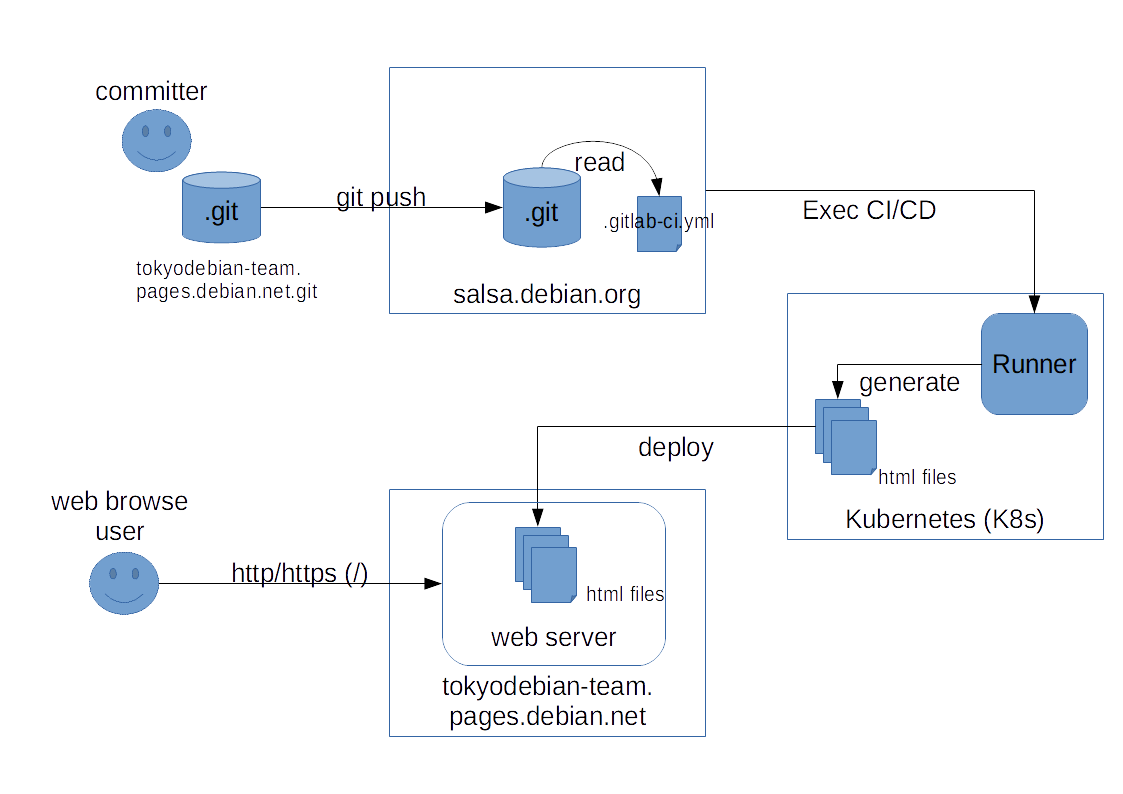
\includegraphics[width=12cm]{image201806/gitflow_web.png}
  \caption{web$B%5%$%H$X(BHTML$B%U%!%$%k$rG[Hw$9$k(BCI/CD$B=hM}$NN.$l(B}
  \label{fig:deploy-html-CICD}
\end{center}
\end{figure}


\subsubsection{$B869F%7%9%F%`$N;EAH$_(B}

$BEl5~%(%j%"(BDebian$BJY6/2q$N869F;qNA$*$h$S%9%i%$%I;qNA$N%=!<%9%3!<%I$O!"(B\url{https://salsa.debian.org/tokyodebian-team/monthly-report} $B$N%Z!<%8$K$"$j$^$9(B\footnote{$B4X@>(BDebian$BJY6/2q$N;qNA$b$3$3$K$"$j$^$9!#(B}$B!#(B


$B%3%s%F%s%D$O(BTeX$B!J%F%U!K$H$$$&AHHG%7%9%F%`(B\footnote{$B0u:~$rA[Dj$7$?%l%$%"%&%H$dJ8;z!"?^$J$I$rG[CV$7$F869F$r:n@.$9$k%7%9%F%`$N$3$H$r$$$$$^$9!#(B}$B$rMxMQ$7$F$*$j!"%=!<%9%3!<%I$G$"$k(Btex$B%U%!%$%k$+$iCf4V%U%!%$%k$N(Bdvi$B%U%!%$%k$r7P$F!":G=*E*$K(Bpdf$B%U%!%$%k$r@8@.$9$k;EAH$_$K$J$C$F$$$^$9!#G[I[$7$F$$$k;qNA$O!"(Btex$B$N%F%s%W%l!<%H$rJY6/2q$NM-;V$,:n@.$7!"K-IY$J869F$NNL$O;22C<T$ND9G/$N@Q$_=E$M$G;Y$($i$l$F$$$^$9!#(B


salsa$B$G$O!"(Btex$B%U%!%$%k$rJ]B8$9$k(Bgit$B%j%]%8%H%j(B"monthly-report.git"$B$H!"(Bweb$B8x3+$9$k%S%k%I$7$?(Bpdf$B%U%!%$%k$rJ]B8$9$k(B"pdf20yy.git"$B$H$$$&%j%]%8%H%j$KJ,$1$F$$$^$9(B\footnote{"pdf20xx.git"$B$O!"(B"pdf2005.git"$B$+$i(B"pdf2018.git"$B$^$GB8:_$7$F$*$j!"KhG/A}$($kM=Dj$G$9!#(B}$B!#$3$l$O!"(B"monthly-report.git"$B$G(Btex$B%U%!%$%k$r(BCI/CD$B$NEY$K$9$Y$F%S%k%I$7D>$9$K$O=hM}NL$,B?$9$.$k$3$H!"(BCI/CD$B=hM}$,@.8y$7$?$H$7$F$b(Bpdf$B%U%!%$%k?t$,B?$9$.$F%5!<%P4V$N(BHTTP$BDL?.$NAw?.2DG=%5%$%:$N>e8B$rD6$($F%(%i!<$K$J$k$3$H$+$i(B\footnote{ERROR: Uploading artifacts to coordinator... too large archive id=11633 responseStatus=413 Request Entity Too Large status=413 Request Entity Too Large token=5ydbgD39}$B!"0lEY$N(BCI/CD$B$G=hM}$9$k(Bpdf$B%U%!%$%k$NNL$r@)8B$9$k$?$a$K%j%]%8%H%j$rG/$4$H$KJ,3d$7$?7P0^$,$"$j$^$9!#(B


$B>e5-$NE>Aw%U%!%$%k%5%$%:$N@)Ls$r2sHr$9$k$?$a!"(Bsalsa$B$K$*$1$k869F%U%!%$%k$N@8@.$+$i(Bpdf$B%U%!%$%k$r(Bweb$B8x3+$9$k$^$G$N=hM}$O0J2<$KN.$l$K$J$C$F$$$^$9!#(B


\begin{itemize}
  \item tex$B%U%!%$%k$rJ]B8$7$F$$$k(B"monthly-report.git"$B$r(Bgit clone$B$7$F(Btex$B%U%!%$%k$r:n@.$9$k(B
  \item make$B$r<B9T$7!"(Bpdf$B%U%!%$%k$,@8@.$G$-$k$3$H$r3NG'$9$k(B
  \item $B869F$r40@.$5$;$k(B
  \item tex$B%U%!%$%k$r(Bgit commit$B$7!"(Bgit push$B$9$k!#(Bpush$B;~$K(Bsalsa$B$G$O(BCI/CD$B=hM}$O<B9T$7$J$$(B
  \item make publish$B%3%^%s%I$r<B9T$7!"(Bpdf$B%U%!%$%k$r(B"pdf20yy.git"$B$X(Bgit commit$B$7!"(Bgit push$B$9$k(B
  \item "pdf20yy.git"$B$G(BCI/CD$B=hM}$r<B9T$7!"(Bpdf$B%U%!%$%k$r(B"tokyodebian-team.pages.debian.net"$B$KG[Hw$9$k(B
  \item web$B$+$i(B"https://tokyodebian-team.pages.debian.net/pdf20yy/xxx.pdf"$B$G%U%!%$%k$r<hF@$G$-$k(B
\end{itemize}


\begin{figure}[H]
\begin{center}
  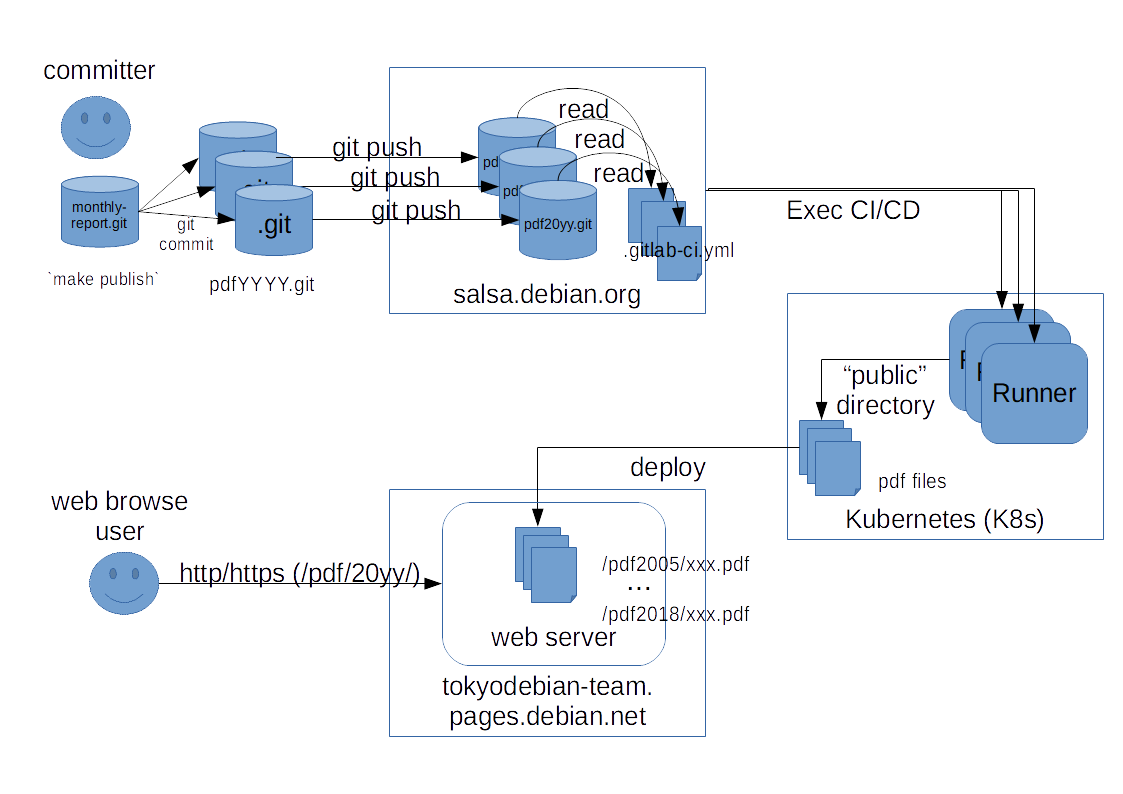
\includegraphics[width=12cm]{image201806/gitflow_pdf.png}
  \caption{web$B%5%$%H$X869F5Z$S%9%i%$%I(BPDF$B%U%!%$%k$rG[Hw$9$k(BCI/CD$B=hM}$NN.$l(B}
  \label{fig:deploy-pdf-CICD}
\end{center}
\end{figure}


\subsection{$B:#8e$N2]Bj(B}

$B869F%7%9%F%`$N(BCI/CD$B=hM}$,<:GT$9$k$3$H$b$"$j!"(BRunner$B$d(B.gitlab-ci.yml$B$N@_Dj$r8+D>$9I,MW$,$"$k$H9M$($F$$$^$9!#(B

web$B%5%$%H$b869F%7%9%F%`$b:n$C$F$+$iG/7n$,7P2a$7$F$$$k$?$a!"(Bweb$B%5%$%H$N%j%K%e!<%"%k$d869F%U%!%$%k$N(BUTF-8$BBP1~$H$$$C$?8=Be2=$r$7$F$$$/=E$a$N2~=$:n6H$b$"$j$^$9!#(B

$B$^$?JY6/2q$GH/I=$7$F$$$?$@$$$F$$$kJ}!9$bK;$7$$$?$a$+869F$r=q$$$F$$$?$@$1$kJ}$,8:$C$F$*$j!"H>4|$N$^$H$a;qNA$r:};R$K$7$?$H$-$K%Z!<%8?t$,>/$J$/$J$C$F$-$F$$$k<B>p$b$"$j$^$9!#(B


\subsection{$B$^$H$a(B}

salsa$B$GDs6!$7$F$$$k(Bgitlab$B$N5!G=$H@_Dj$r>R2p$7!"$=$N5!G=$r;H$C$FEl5~%(%j%"(BDebian$BJY6/2q$N%7%9%F%`$r0\9T$7$?@bL@$r$7$^$7$?!#(Bsalsa$B$rM-8z3hMQ$7$F(BDebian$B%W%m%8%'%/%H$X9W8%$9$k$3$H$K7R$,$k$H$h$$$H;W$C$F$$$^$9!#(B

$B$^$?!"JY6/2q$N;22C<T$K869F%7%9%F%`$NM}2r$r?<$a$F$$$?$@$-!"<+J,$N3X$S$K$J$k$@$1$G$J$/!"B>$N;22C<T$d%$%s%?!<%M%C%H$G8!:w$7$F$-$?J}$N3X$S$K$D$J$,$kJY6/2q$K$7$F$$$1$l$P$h$$$H;W$C$F$$$^$9!#(B

%-------------------------------------------------------------------------------
% end of header
%-------------------------------------------------------------------------------

\clearpage
\newpage

%-------------------------------------------------------------------------------
%\dancersection{Debian Trivia Quiz}{$BLnEg(B $B5.1Q(B}
%-------------------------------------------------------------------------------

%$B$H$3$m$G!"$_$J$5$s(B Debian $B4XO"$NOCBj$K$*$$$D$$$F$$$^$9$+!)(BDebian$B4XO"$NOC(B
%$BBj$O%a!<%j%s%0%j%9%H$r$h$s$G$$$k$HDI@W$G$-$^$9!#$?$@$h$s$G$$$k$@$1$G$O$O(B
%$B$j$"$$$,$J$$$N$G!"M}2rEY$N%F%9%H$r$7$^$9!#FC$K0l?M$@$1$G$O0UL#$,$o$+$i$J(B
%$B$$$H$3$m$b$"$k$+$bCN$l$^$;$s!#$_$s$J$G0l=o$KFI$s$G$_$^$7$g$&!#(B

%$B:#2s$N=PBjHO0O$O(B\url{debian-devel-announce@lists.debian.org} $B$d(B \url{debian-devel@lists.debian.org}$B$KEj9F$5$l$?(B
%$BFbMF$H(BDebian Project News$B$+$i$G$9!#(B

%\begin{multicols}{2}
%\end{multicols}

% $B:w0z(B
%\printindex
\clearpage
\begin{center}
$BK\;qNA$N%i%$%;%s%9$K$D$$$F(B
\end{center}

$BK\;qNA$O%U%j!<!&%=%U%H%&%'%"$G$9!#$"$J$?$O!"(BFree Software
Foundation $B$,8xI=$7$?(BGNU GENERAL PUBLIC LICENSE$B$N(B "$B%P!<%8%g%s#2(B"$B$b$7$/$O$=$l0J9_(B
$B$,Dj$a$k>r9`$K=>$C$FK\%W%m%0%i%`$r:FHRI[$^$?$OJQ99$9$k$3$H$,$G$-(B
$B$^$9!#(B

$BK\%W%m%0%i%`$OM-MQ$H$O;W$$$^$9$,!"HRI[$K$"$?$C$F$O!";T>l@-5Z$SFC(B
$BDjL\E*E,9g@-$K$D$$$F$N0EL[$NJ]>Z$r4^$a$F!"$$$+$J$kJ]>Z$b9T$J$$$^(B
$B$;$s!#>\:Y$K$D$$$F$O(BGNU GENERAL PUBLIC LICENSE $B$r$*FI$_$/$@$5$$!#(B

\begin{multicols}{2}
 \begin{fontsize}{6}{6}
 \begin{verbatim}
            GNU GENERAL PUBLIC LICENSE
               Version 2, June 1991

 Copyright (C) 1989, 1991 Free Software Foundation, Inc.
    51 Franklin St, Fifth Floor, Boston, MA  02110-1301  USA
 Everyone is permitted to copy and distribute verbatim copies
 of this license document, but changing it is not allowed.

                Preamble

  The licenses for most software are designed to take away your
freedom to share and change it.  By contrast, the GNU General Public
License is intended to guarantee your freedom to share and change free
software--to make sure the software is free for all its users.  This
General Public License applies to most of the Free Software
Foundation's software and to any other program whose authors commit to
using it.  (Some other Free Software Foundation software is covered by
the GNU Library General Public License instead.)  You can apply it to
your programs, too.

  When we speak of free software, we are referring to freedom, not
price.  Our General Public Licenses are designed to make sure that you
have the freedom to distribute copies of free software (and charge for
this service if you wish), that you receive source code or can get it
if you want it, that you can change the software or use pieces of it
in new free programs; and that you know you can do these things.

  To protect your rights, we need to make restrictions that forbid
anyone to deny you these rights or to ask you to surrender the rights.
These restrictions translate to certain responsibilities for you if you
distribute copies of the software, or if you modify it.

  For example, if you distribute copies of such a program, whether
gratis or for a fee, you must give the recipients all the rights that
you have.  You must make sure that they, too, receive or can get the
source code.  And you must show them these terms so they know their
rights.

  We protect your rights with two steps: (1) copyright the software, and
(2) offer you this license which gives you legal permission to copy,
distribute and/or modify the software.

  Also, for each author's protection and ours, we want to make certain
that everyone understands that there is no warranty for this free
software.  If the software is modified by someone else and passed on, we
want its recipients to know that what they have is not the original, so
that any problems introduced by others will not reflect on the original
authors' reputations.

  Finally, any free program is threatened constantly by software
patents.  We wish to avoid the danger that redistributors of a free
program will individually obtain patent licenses, in effect making the
program proprietary.  To prevent this, we have made it clear that any
patent must be licensed for everyone's free use or not licensed at all.

  The precise terms and conditions for copying, distribution and
modification follow.

            GNU GENERAL PUBLIC LICENSE
   TERMS AND CONDITIONS FOR COPYING, DISTRIBUTION AND MODIFICATION

  0. This License applies to any program or other work which contains
a notice placed by the copyright holder saying it may be distributed
under the terms of this General Public License.  The "Program", below,
refers to any such program or work, and a "work based on the Program"
means either the Program or any derivative work under copyright law:
that is to say, a work containing the Program or a portion of it,
either verbatim or with modifications and/or translated into another
language.  (Hereinafter, translation is included without limitation in
the term "modification".)  Each licensee is addressed as "you".

Activities other than copying, distribution and modification are not
covered by this License; they are outside its scope.  The act of
running the Program is not restricted, and the output from the Program
is covered only if its contents constitute a work based on the
Program (independent of having been made by running the Program).
Whether that is true depends on what the Program does.

  1. You may copy and distribute verbatim copies of the Program's
source code as you receive it, in any medium, provided that you
conspicuously and appropriately publish on each copy an appropriate
copyright notice and disclaimer of warranty; keep intact all the
notices that refer to this License and to the absence of any warranty;
and give any other recipients of the Program a copy of this License
along with the Program.

You may charge a fee for the physical act of transferring a copy, and
you may at your option offer warranty protection in exchange for a fee.

  2. You may modify your copy or copies of the Program or any portion
of it, thus forming a work based on the Program, and copy and
distribute such modifications or work under the terms of Section 1
above, provided that you also meet all of these conditions:

    a) You must cause the modified files to carry prominent notices
    stating that you changed the files and the date of any change.

    b) You must cause any work that you distribute or publish, that in
    whole or in part contains or is derived from the Program or any
    part thereof, to be licensed as a whole at no charge to all third
    parties under the terms of this License.

    c) If the modified program normally reads commands interactively
    when run, you must cause it, when started running for such
    interactive use in the most ordinary way, to print or display an
    announcement including an appropriate copyright notice and a
    notice that there is no warranty (or else, saying that you provide
    a warranty) and that users may redistribute the program under
    these conditions, and telling the user how to view a copy of this
    License.  (Exception: if the Program itself is interactive but
    does not normally print such an announcement, your work based on
    the Program is not required to print an announcement.)

These requirements apply to the modified work as a whole.  If
identifiable sections of that work are not derived from the Program,
and can be reasonably considered independent and separate works in
themselves, then this License, and its terms, do not apply to those
sections when you distribute them as separate works.  But when you
distribute the same sections as part of a whole which is a work based
on the Program, the distribution of the whole must be on the terms of
this License, whose permissions for other licensees extend to the
entire whole, and thus to each and every part regardless of who wrote it.

Thus, it is not the intent of this section to claim rights or contest
your rights to work written entirely by you; rather, the intent is to
exercise the right to control the distribution of derivative or
collective works based on the Program.

In addition, mere aggregation of another work not based on the Program
with the Program (or with a work based on the Program) on a volume of
a storage or distribution medium does not bring the other work under
the scope of this License.

  3. You may copy and distribute the Program (or a work based on it,
under Section 2) in object code or executable form under the terms of
Sections 1 and 2 above provided that you also do one of the following:

    a) Accompany it with the complete corresponding machine-readable
    source code, which must be distributed under the terms of Sections
    1 and 2 above on a medium customarily used for software interchange; or,

    b) Accompany it with a written offer, valid for at least three
    years, to give any third party, for a charge no more than your
    cost of physically performing source distribution, a complete
    machine-readable copy of the corresponding source code, to be
    distributed under the terms of Sections 1 and 2 above on a medium
    customarily used for software interchange; or,

    c) Accompany it with the information you received as to the offer
    to distribute corresponding source code.  (This alternative is
    allowed only for noncommercial distribution and only if you
    received the program in object code or executable form with such
    an offer, in accord with Subsection b above.)

The source code for a work means the preferred form of the work for
making modifications to it.  For an executable work, complete source
code means all the source code for all modules it contains, plus any
associated interface definition files, plus the scripts used to
control compilation and installation of the executable.  However, as a
special exception, the source code distributed need not include
anything that is normally distributed (in either source or binary
form) with the major components (compiler, kernel, and so on) of the
operating system on which the executable runs, unless that component
itself accompanies the executable.

If distribution of executable or object code is made by offering
access to copy from a designated place, then offering equivalent
access to copy the source code from the same place counts as
distribution of the source code, even though third parties are not
compelled to copy the source along with the object code.

  4. You may not copy, modify, sublicense, or distribute the Program
except as expressly provided under this License.  Any attempt
otherwise to copy, modify, sublicense or distribute the Program is
void, and will automatically terminate your rights under this License.
However, parties who have received copies, or rights, from you under
this License will not have their licenses terminated so long as such
parties remain in full compliance.

  5. You are not required to accept this License, since you have not
signed it.  However, nothing else grants you permission to modify or
distribute the Program or its derivative works.  These actions are
prohibited by law if you do not accept this License.  Therefore, by
modifying or distributing the Program (or any work based on the
Program), you indicate your acceptance of this License to do so, and
all its terms and conditions for copying, distributing or modifying
the Program or works based on it.

  6. Each time you redistribute the Program (or any work based on the
Program), the recipient automatically receives a license from the
original licensor to copy, distribute or modify the Program subject to
these terms and conditions.  You may not impose any further
restrictions on the recipients' exercise of the rights granted herein.
You are not responsible for enforcing compliance by third parties to
this License.

  7. If, as a consequence of a court judgment or allegation of patent
infringement or for any other reason (not limited to patent issues),
conditions are imposed on you (whether by court order, agreement or
otherwise) that contradict the conditions of this License, they do not
excuse you from the conditions of this License.  If you cannot
distribute so as to satisfy simultaneously your obligations under this
License and any other pertinent obligations, then as a consequence you
may not distribute the Program at all.  For example, if a patent
license would not permit royalty-free redistribution of the Program by
all those who receive copies directly or indirectly through you, then
the only way you could satisfy both it and this License would be to
refrain entirely from distribution of the Program.

If any portion of this section is held invalid or unenforceable under
any particular circumstance, the balance of the section is intended to
apply and the section as a whole is intended to apply in other
circumstances.

It is not the purpose of this section to induce you to infringe any
patents or other property right claims or to contest validity of any
such claims; this section has the sole purpose of protecting the
integrity of the free software distribution system, which is
implemented by public license practices.  Many people have made
generous contributions to the wide range of software distributed
through that system in reliance on consistent application of that
system; it is up to the author/donor to decide if he or she is willing
to distribute software through any other system and a licensee cannot
impose that choice.

This section is intended to make thoroughly clear what is believed to
be a consequence of the rest of this License.

  8. If the distribution and/or use of the Program is restricted in
certain countries either by patents or by copyrighted interfaces, the
original copyright holder who places the Program under this License
may add an explicit geographical distribution limitation excluding
those countries, so that distribution is permitted only in or among
countries not thus excluded.  In such case, this License incorporates
the limitation as if written in the body of this License.

  9. The Free Software Foundation may publish revised and/or new versions
of the General Public License from time to time.  Such new versions will
be similar in spirit to the present version, but may differ in detail to
address new problems or concerns.

Each version is given a distinguishing version number.  If the Program
specifies a version number of this License which applies to it and "any
later version", you have the option of following the terms and conditions
either of that version or of any later version published by the Free
Software Foundation.  If the Program does not specify a version number of
this License, you may choose any version ever published by the Free Software
Foundation.

  10. If you wish to incorporate parts of the Program into other free
programs whose distribution conditions are different, write to the author
to ask for permission.  For software which is copyrighted by the Free
Software Foundation, write to the Free Software Foundation; we sometimes
make exceptions for this.  Our decision will be guided by the two goals
of preserving the free status of all derivatives of our free software and
of promoting the sharing and reuse of software generally.

                NO WARRANTY

  11. BECAUSE THE PROGRAM IS LICENSED FREE OF CHARGE, THERE IS NO WARRANTY
FOR THE PROGRAM, TO THE EXTENT PERMITTED BY APPLICABLE LAW.  EXCEPT WHEN
OTHERWISE STATED IN WRITING THE COPYRIGHT HOLDERS AND/OR OTHER PARTIES
PROVIDE THE PROGRAM "AS IS" WITHOUT WARRANTY OF ANY KIND, EITHER EXPRESSED
OR IMPLIED, INCLUDING, BUT NOT LIMITED TO, THE IMPLIED WARRANTIES OF
MERCHANTABILITY AND FITNESS FOR A PARTICULAR PURPOSE.  THE ENTIRE RISK AS
TO THE QUALITY AND PERFORMANCE OF THE PROGRAM IS WITH YOU.  SHOULD THE
PROGRAM PROVE DEFECTIVE, YOU ASSUME THE COST OF ALL NECESSARY SERVICING,
REPAIR OR CORRECTION.

  12. IN NO EVENT UNLESS REQUIRED BY APPLICABLE LAW OR AGREED TO IN WRITING
WILL ANY COPYRIGHT HOLDER, OR ANY OTHER PARTY WHO MAY MODIFY AND/OR
REDISTRIBUTE THE PROGRAM AS PERMITTED ABOVE, BE LIABLE TO YOU FOR DAMAGES,
INCLUDING ANY GENERAL, SPECIAL, INCIDENTAL OR CONSEQUENTIAL DAMAGES ARISING
OUT OF THE USE OR INABILITY TO USE THE PROGRAM (INCLUDING BUT NOT LIMITED
TO LOSS OF DATA OR DATA BEING RENDERED INACCURATE OR LOSSES SUSTAINED BY
YOU OR THIRD PARTIES OR A FAILURE OF THE PROGRAM TO OPERATE WITH ANY OTHER
PROGRAMS), EVEN IF SUCH HOLDER OR OTHER PARTY HAS BEEN ADVISED OF THE
POSSIBILITY OF SUCH DAMAGES.

             END OF TERMS AND CONDITIONS

        How to Apply These Terms to Your New Programs

  If you develop a new program, and you want it to be of the greatest
possible use to the public, the best way to achieve this is to make it
free software which everyone can redistribute and change under these terms.

  To do so, attach the following notices to the program.  It is safest
to attach them to the start of each source file to most effectively
convey the exclusion of warranty; and each file should have at least
the "copyright" line and a pointer to where the full notice is found.

    <one line to give the program's name and a brief idea of what it does.>
    Copyright (C) <year>  <name of author>

    This program is free software; you can redistribute it and/or modify
    it under the terms of the GNU General Public License as published by
    the Free Software Foundation; either version 2 of the License, or
    (at your option) any later version.

    This program is distributed in the hope that it will be useful,
    but WITHOUT ANY WARRANTY; without even the implied warranty of
    MERCHANTABILITY or FITNESS FOR A PARTICULAR PURPOSE.  See the
    GNU General Public License for more details.

    You should have received a copy of the GNU General Public License
    along with this program; if not, write to the Free Software
    Foundation, Inc., 51 Franklin St, Fifth Floor, Boston, MA  02110-1301 USA


Also add information on how to contact you by electronic and paper mail.

If the program is interactive, make it output a short notice like this
when it starts in an interactive mode:

    Gnomovision version 69, Copyright (C) year  name of author
    Gnomovision comes with ABSOLUTELY NO WARRANTY; for details type `show w'.
    This is free software, and you are welcome to redistribute it
    under certain conditions; type `show c' for details.

The hypothetical commands `show w' and `show c' should show the appropriate
parts of the General Public License.  Of course, the commands you use may
be called something other than `show w' and `show c'; they could even be
mouse-clicks or menu items--whatever suits your program.

You should also get your employer (if you work as a programmer) or your
school, if any, to sign a "copyright disclaimer" for the program, if
necessary.  Here is a sample; alter the names:

  Yoyodyne, Inc., hereby disclaims all copyright interest in the program
  `Gnomovision' (which makes passes at compilers) written by James Hacker.

  <signature of Ty Coon>, 1 April 1989
  Ty Coon, President of Vice

This General Public License does not permit incorporating your program into
proprietary programs.  If your program is a subroutine library, you may
consider it more useful to permit linking proprietary applications with the
library.  If this is what you want to do, use the GNU Library General
Public License instead of this License.
 \end{verbatim}
 \end{fontsize}
\end{multicols}

\begin{center}
$B%=!<%9%3!<%I$K$D$$$F(B
\end{center}

$B$3$N%W%m%0%i%`$O(B tex $B$G5-=R$5$l$?$b$N$G$9!#%=!<%9%3!<%I$O(B
\begin{center}
  \url{git://anonscm.debian.org/tokyodebian/monthly-report.git}
\end{center}
$B$+$i<hF@$G$-$^$9!#(B

\begin{center}
Debian $B%*!<%W%s%f!<%:%m%4(B $B%i%$%;%s%9(B
\end{center}

\begin{multicols}{2}
 \begin{fontsize}{6}{6}
 \begin{verbatim}

Copyright (c) 1999 Software in the Public Interest
Permission is hereby granted, free of charge, to any person
obtaining a copy of this software and associated documentation
files (the "Software"), to deal in the Software without restriction,
including without limitation the rights to use, copy, modify, merge,
publish, distribute, sublicense, and/or sell copies of the Software,
and to permit persons to whom the Software is furnished to do so,
subject to the following conditions:

The above copyright notice and this permission notice shall be
included in all copies or substantial portions of the Software.

THE SOFTWARE IS PROVIDED "AS IS", WITHOUT WARRANTY OF ANY
KIND, EXPRESS OR IMPLIED, INCLUDING BUT NOT LIMITED TO THE
WARRANTIES OF MERCHANTABILITY, FITNESS FOR A PARTICULAR PURPOSE AND
NONINFRINGEMENT. IN NO EVENT SHALL THE AUTHORS OR COPYRIGHT HOLDERS
BE LIABLE FOR ANY CLAIM, DAMAGES OR OTHER LIABILITY, WHETHER IN
AN ACTION OF CONTRACT, TORT OR OTHERWISE, ARISING FROM, OUT OF OR
IN CONNECTION WITH THE SOFTWARE OR THE USE OR OTHER DEALINGS IN
THE SOFTWARE.
 \end{verbatim}
 \end{fontsize}
\end{multicols}

% $BLdBj$H2sEz$,F1$8$_$R$i$-$K$J$i$J$$$h$&$K$9$k(B
%\cleartoevenpage
%-------------------------------------------------------------------------------
%\dancersection{Debian Trivia Quiz $BLdBj2sEz(B}{ }
%-------------------------------------------------------------------------------
%\\
%{\small
% Debian Trivia Quiz $B$NLdBj2sEz$G$9!#(B $B$"$J$?$O2?Ld$o$+$j$^$7$?$+!)(B \\
 %$B2sEz$O(Bdebianmeetingresume2016-natsu.jqz$B$H$$$&%U%!%$%k$K@8@.$5$l$k$N$G!"(B
 %$B$=$l$r<jF0$G%3%T%Z$7$F;H$&!#(B
 % $B$3$3$+$i%3%T%Z(B
 % FIXME $BLdBj$,A4It$O$$$C$?$i%3%T%Z$9$k$3$H(B
\pagestyle{empty}
\cleartoevenpage
$B!!(B
\pagestyle{empty}
\cleartoevenpage

\newpage
{
\large
\begin{itembox}{\bf $B!X$"$s$I$-$e$a$s$F$C$I(B $B$G$S$"$s!Y$K$D$$$F(B}
% FIXME: $BBP>]$r=$@5$9$k$3$H!#(B
$BK\=q$O!"El5~$*$h$S4X@><~JU$GKh7n9T$J$o$l$F$$$k!XEl5~%(%j%"(B Debian $BJY6/2q!Y!J(B2017$BG/(B12$B7n(B-2018$BG/(B6$B7n!K$*$h$S(B
$B!X4X@>(B Debian $BJY6/2q!Y!J(B2017$BG/(B12$B7n(B-2018$BG/(B5$B7n!K$G;HMQ$5$l$?;qNA!&>.%M%?!&I,;&5;$J$I$r0l:}$K$^$H$a$?$b$N$G$9!#(B
$BFbMF$OL5J]>Z!"$D$C$3$_$J$I$,$"$l$PJY6/2q$K$F!#(B
\end{itembox}
}

\vspace*{13cm}
{\color{dancerlightblue}\rule{\hsize}{1mm}}
\vspace{2mm}

\includegraphics[width=2cm]{image200502/openlogo-nd.eps}
\noindent \Large \bf $B$"$s$I$-$e$a$s$F$C$I(B $B$G$S$"$s(B 2018$BG/2F9f(B\\
\noindent \normalfont 2018$BG/(B8$B7n(B10$BF|(B \hspace{5mm}  $B=iHGBh(B1$B:~H/9T(B\\
\noindent \normalfont $BEl5~%(%j%"(B Debian $BJY6/2q(B/$B4X@>%(%j%"(B Debian $BJY6/2q(B $B!JJT=8!&0u:~!&H/9T!K(B\\
{\color{dancerdarkblue}\rule{\hsize}{1mm}}

\end{document}
